\capitulo{5}{Resultados}



En este capítulo se exponen los resultados obtenidos en el conjunto de validación tras entrenar las arquitecturas con las modificaciones planteadas. Tal y como se plantearon en el \Cref{modelos-a-entrenar}, los experimentos han consistido en entrenar $36$ modelos definidos por el producto cartesiano de las opciones: (ResNet50, EfficientNet-B0) como \textit{backbone}, (Atención estándar, Atención \textit{Performer}) como mecanismo de atención, ($1$, $12$, $24$) como número de cabezas de atención, y ([$0$, $1$], [$2$, $5$], [$8$, $11$]) como bloques de atención de los que se toma la salida para que sea la entrada del \textit{decoder}. En este capítulo, además de las métricas que miden la exactitud de las salidas, se presentan también métricas de velocidad de inferencia. Para medir este último grupo de variables, tras comprobar que los resultados numéricos en la salida de los modelos eran idénticos, se emplea precisión mixta para aumentar la velocidad lo máximo posible (\Cref{fig:resultados-mixed-precision}).

\begin{figure}
\begin{minipage}{.45\textwidth}
  \centering
  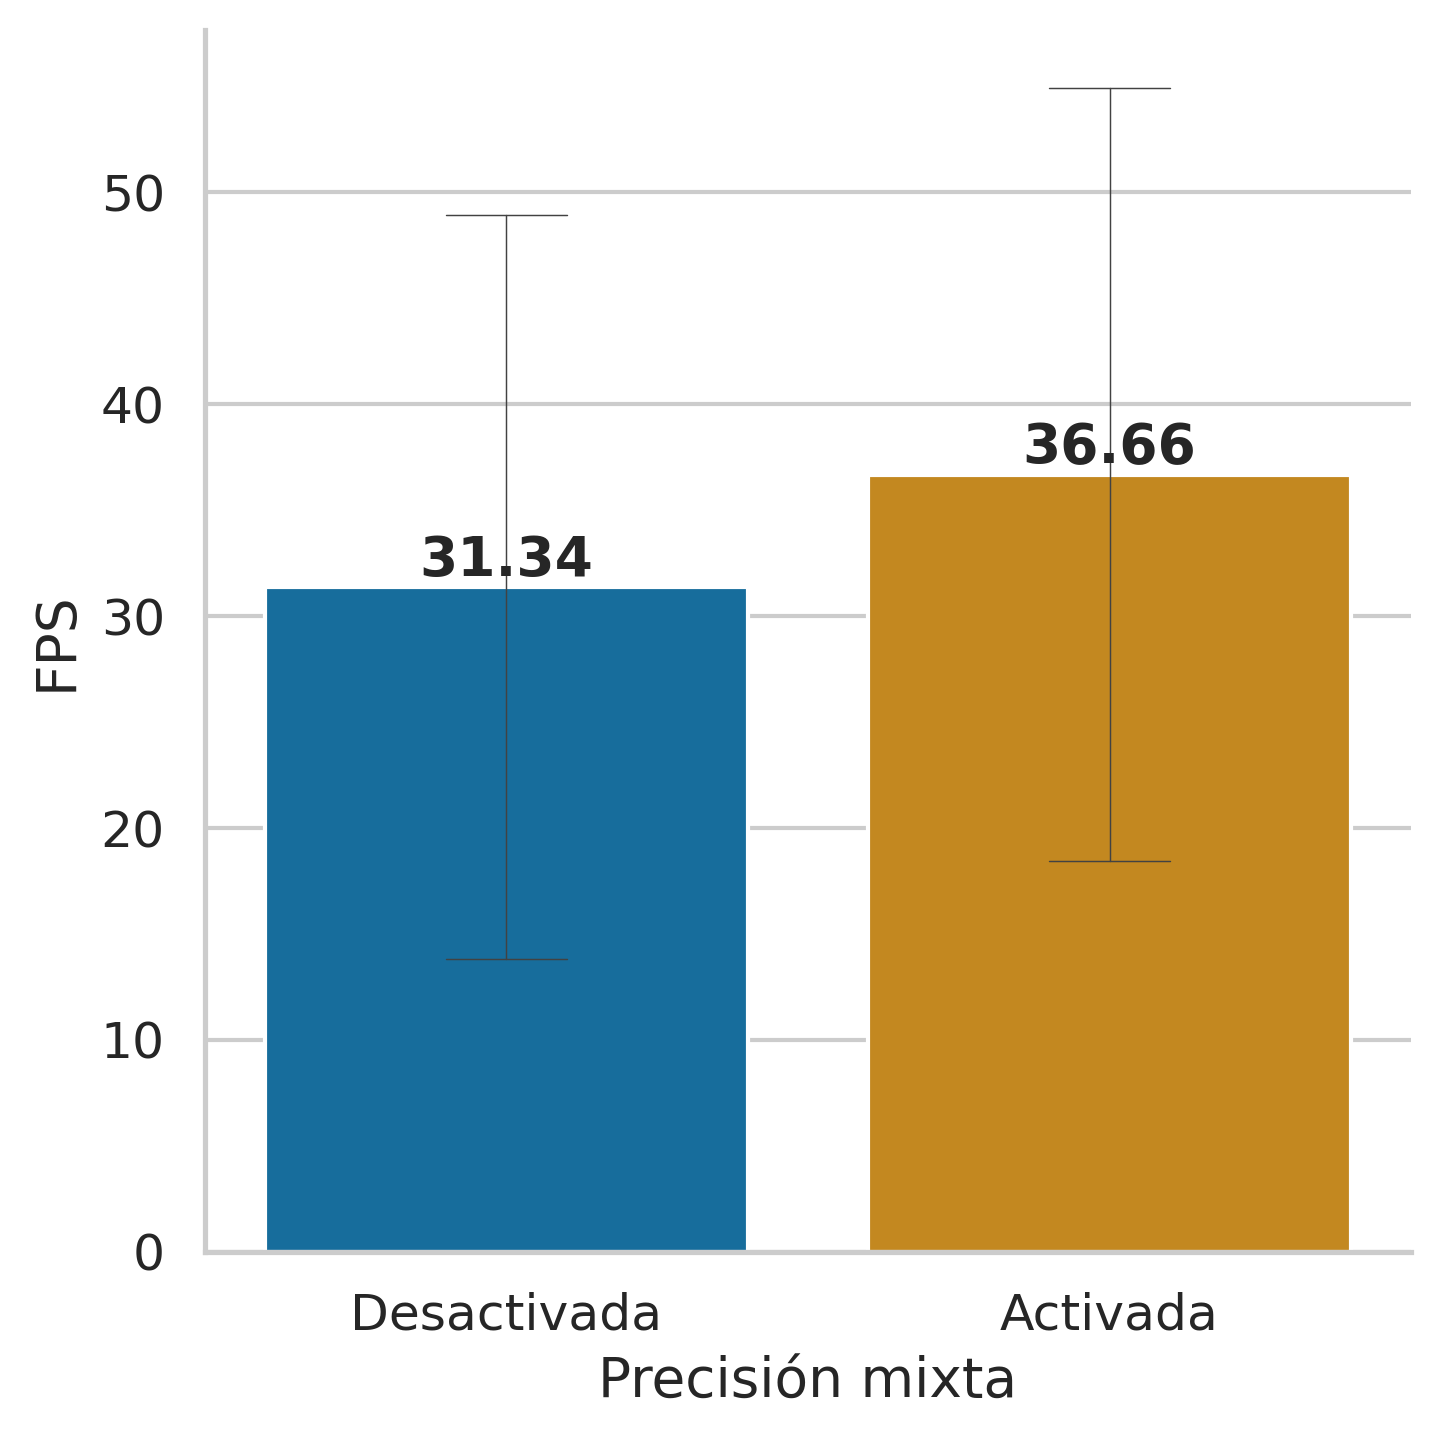
\includegraphics[width=\linewidth]{imagenes/Resultados/mixed_precision.png} 
  \captionof{figure}{FPS promedios de los modelos en función de la precisión durante la inferencia. Las barras grises representan la desviación estándar de las medidas.}
  \label{fig:resultados-mixed-precision}
\end{minipage}%
\hfill
\begin{minipage}{.45\textwidth}
  \centering
  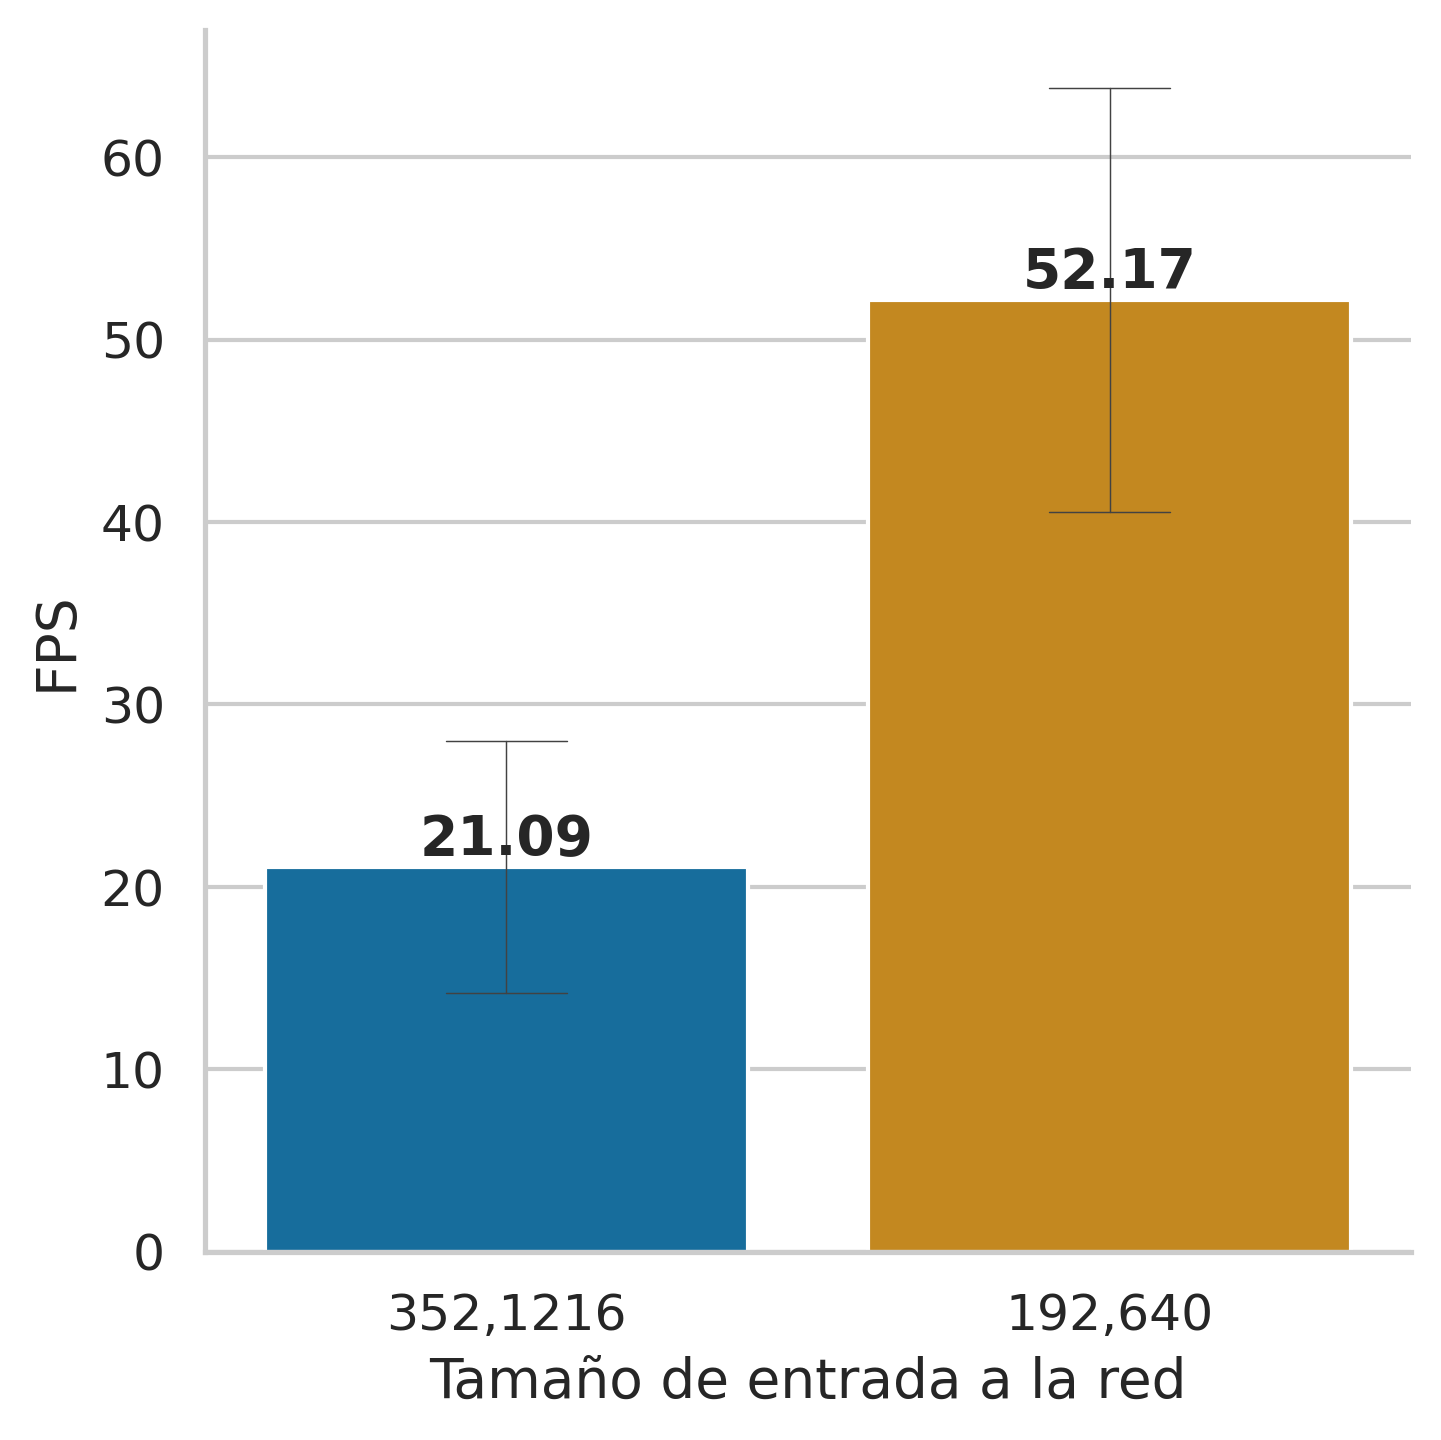
\includegraphics[width=\linewidth]{imagenes/Resultados/velocidad_inferencia_entrada.png} 
  \captionof{figure}{FPS medios de los modelos en función del tamaño de su entrada. Las barras grises representan la desviación estándar de las medidas.}
  \label{fig:resultados-inf-tam-entrada}
\end{minipage}
\end{figure}

\section{Resultados cuantitativos}

\subsection{Reducción del tamaño de la entrada}



Dado que el entrenamientos de los modelos - por limitaciones materiales y temporales - se ha llevado a cabo reduciendo el tamaño de la entrada, no es posible comparar los resultados obtenidos para cada una de las modificaciones de la arquitectura con su modelo entrenado con las imágenes en su tamaño original.

Sin embargo, la medida de la velocidad de inferencia sí que es posible obtenerla independientemente de que los pesos correspondan al modelo entrenado o no. En la \Cref{fig:resultados-inf-tam-entrada} se puede apreciar la diferencia en función del tamaño de entrada de los FPS promedio de todas las modificaciones realizadas sobre el modelo DPT. El valor de la izquierda, corresponde al tamaño con el que se evalúa KITTI en la publicación original \cite{visiontransformersDPT}, mientras que el de la derecha es la reducción de tamaño establecida en este trabajo. Dado que este cambio es significativo y es, en términos de magnitud, el que mayor aceleración media conlleva ($\times2.47$), en las siguientes Figuras que representen los FPS en función de los otros cambios introducidos en el trabajo se presentarán los datos tanto con el tamaño de entrada original como con el tamaño de entrada reducido para poder así valorar también la mejora de rendimiento que conllevaría la modificación si no se hubiese reducido el tamaño de la entrada.



















\subsection{Cambio del backbone convolucional}\label{resultados-cuantitativos-backbone}
El cambio del \textit{backbone} convolucional usado para extraer los mapas de características, como era de esperar, también influye en la velocidad de inferencia de la red. En la \Cref{fig:resultados-inf-backbone}, es posible ver el incremento en los FPS promedio entre los modelos con ResNet50 y los modelos con EfficientNet-B0.

\begin{figure}[H]
\centering
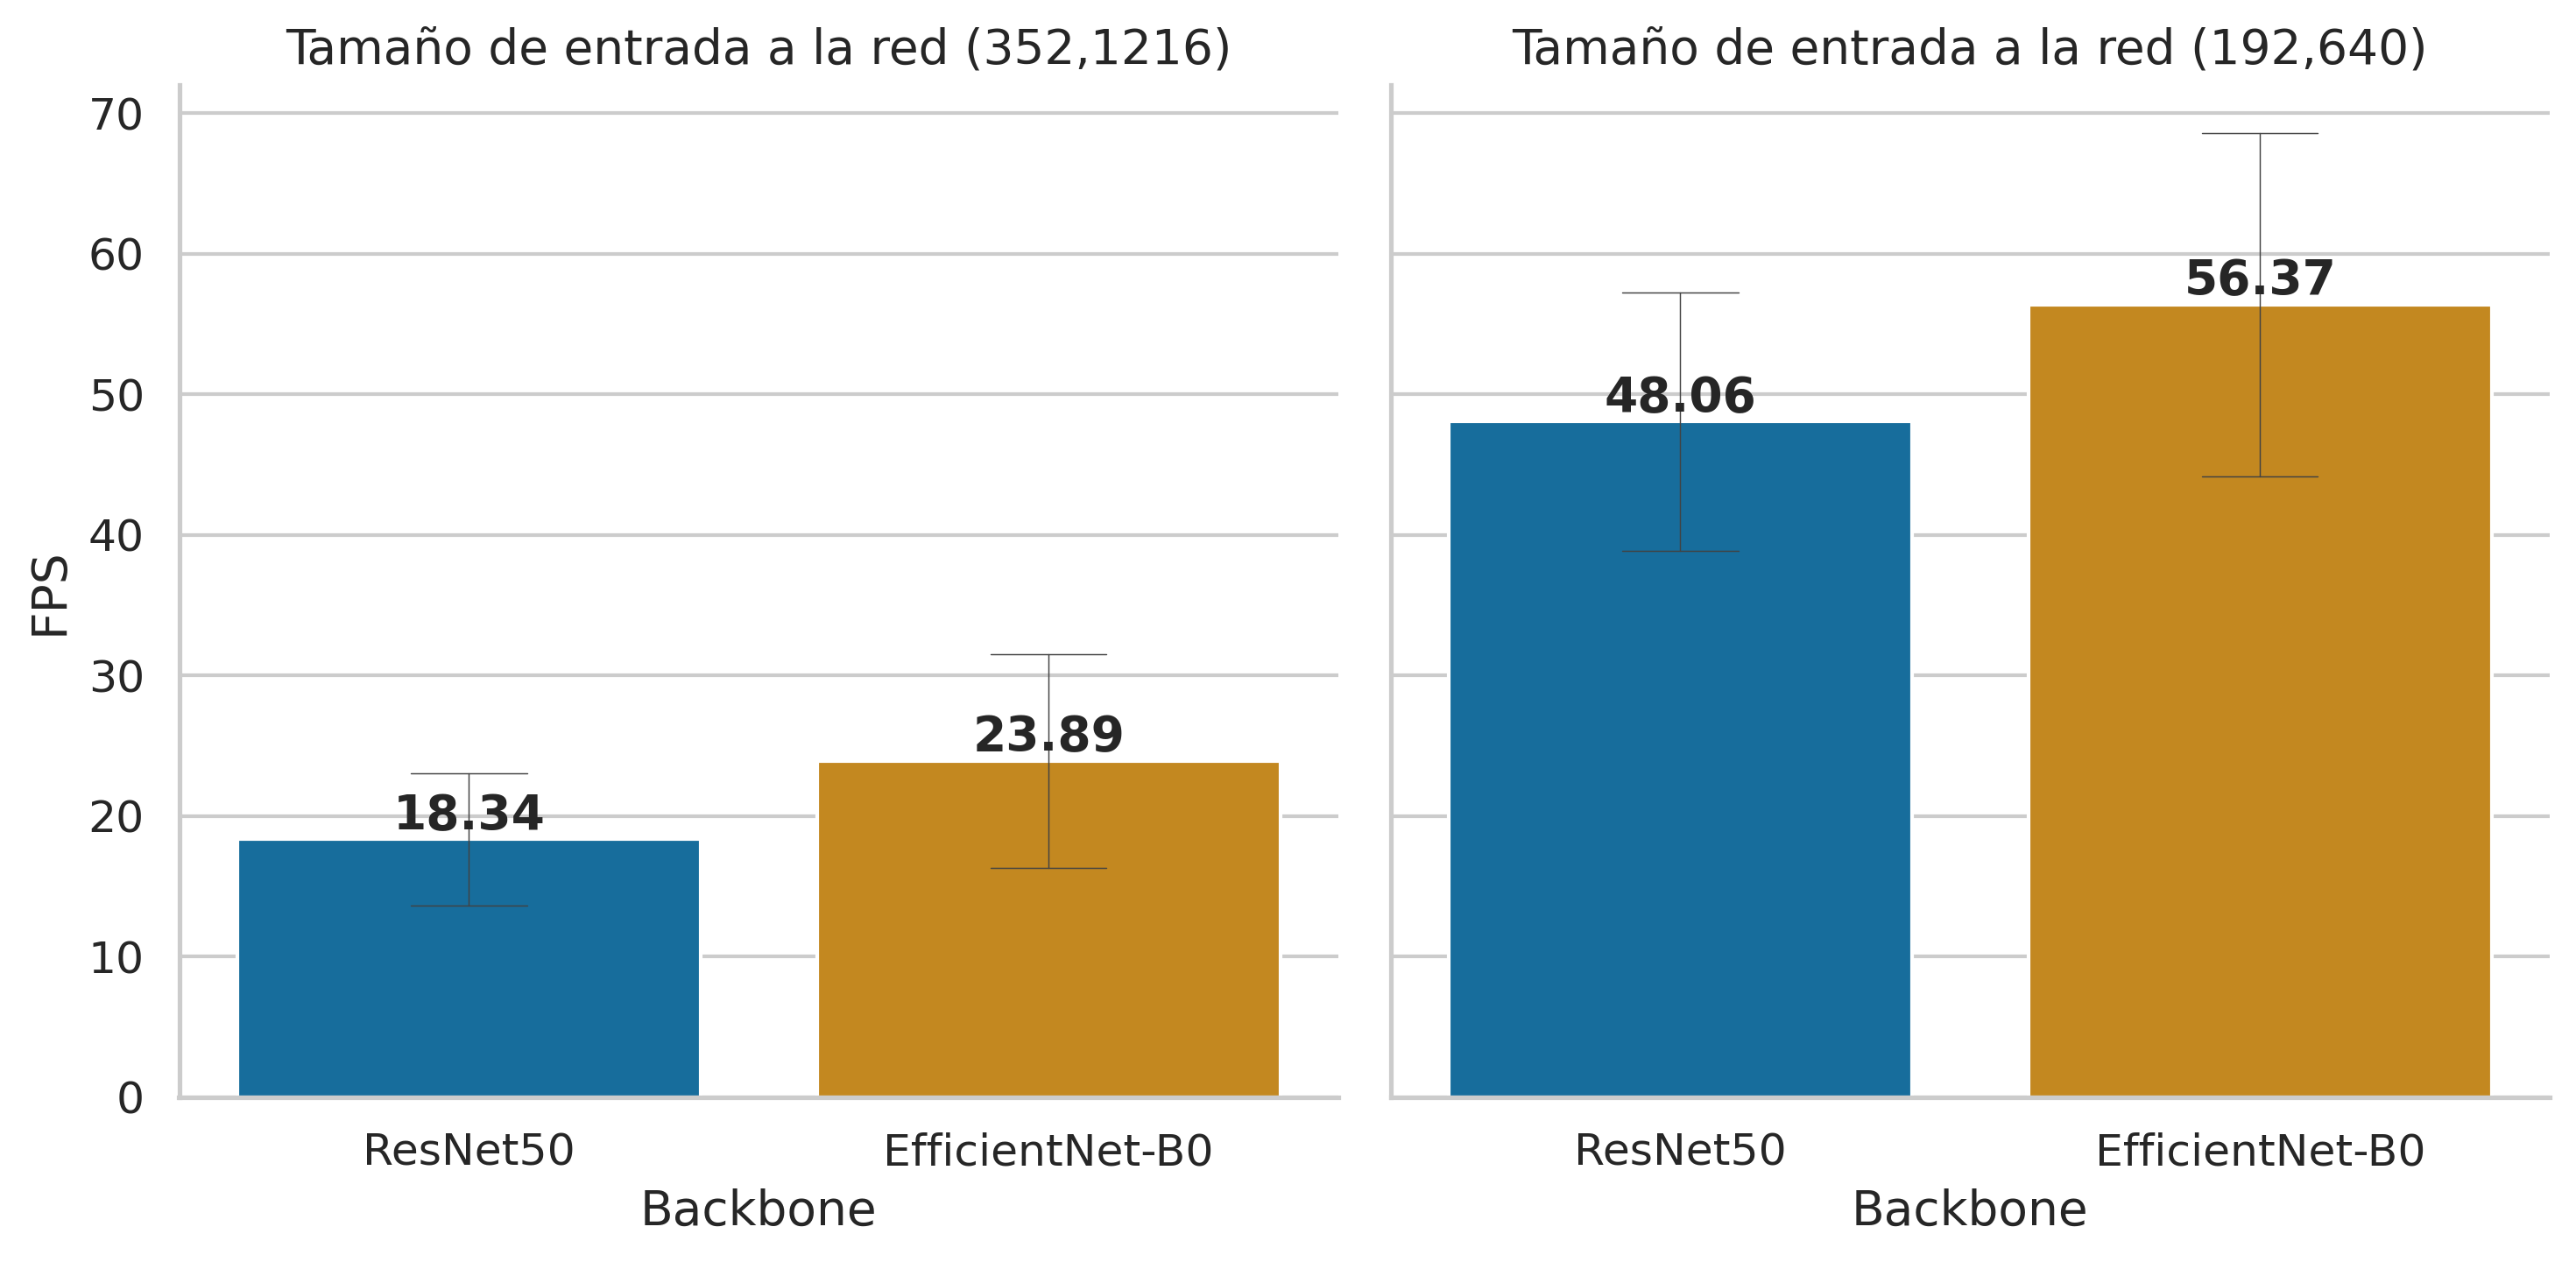
\includegraphics[width=0.8\linewidth]{imagenes/Resultados/velocidad_inferencia_backbone.png} 
\captionsetup{width=.8\linewidth}
\caption{FPS medios de los modelos en función del \textit{backbone} utilizado y del tamaño de la entrada. Las barras grises representan la desviación estándar de las medidas.}
\label{fig:resultados-inf-backbone}
\end{figure}

A pesar de que el incremento de velocidad es positivo, existe un problema asociado a la modificación del \textit{backbone}. De todas las modificaciones desarrolladas y estudiadas en este trabajo, el cambio de \textit{backbone} domina de forma muy considerable el deterioro de la calidad de los resultados, esto se puede ver claramente, por ejemplo, en la comparación del error logarítmico invariante a la escala (SIlog) disponible en la \Cref{fig:SIlog-validation}.

\begin{figure}[H]
\centering
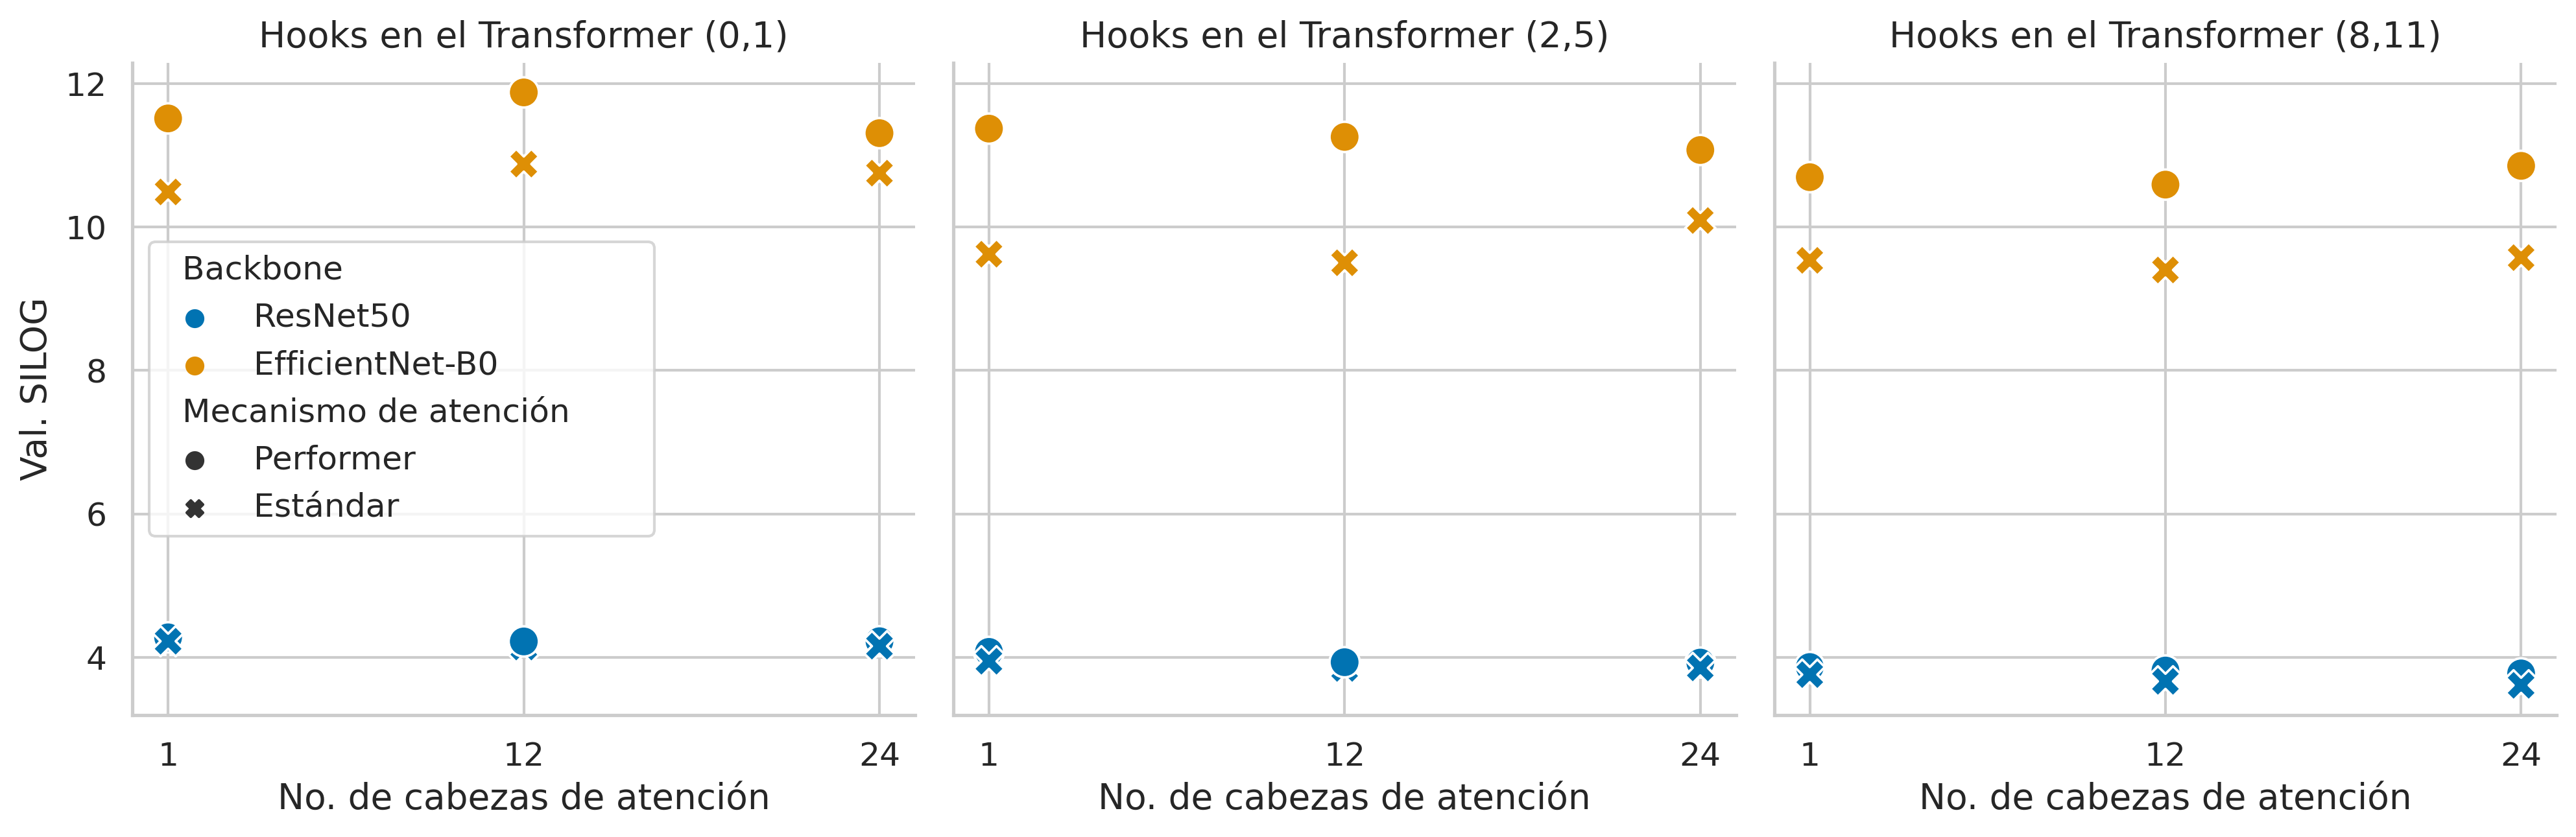
\includegraphics[width=\linewidth]{imagenes/Resultados/SIlog_val.png} 
\captionsetup{width=.95\linewidth}
\caption{SIlog obtenido en el conjunto de validación para cada uno de los 36 modelos entrenados. Más bajo es mejor.}
\label{fig:SIlog-validation}
\end{figure}

Con el objetivo de buscar la causa de esta diferencia tan grande del error, se estudian las curvas de aprendizaje de entrenamiento y validación. En estas curvas (\Cref{fig:efficientnet-overfitting}), se puede observar como en comparación con el modelo equivalente con ResNet50, el modelo que tiene como \textit{backbone} la EfficientNet-B0 está sobreajustando (\textit{overfitting}) sus parámetros al conjunto de entrenamiento, ya que la diferencia entre el error en el conjunto de entrenamiento y el error en el conjunto de validación es mucho mayor en el caso del modelo con EfficientNet.

\begin{figure}[H]
\centering
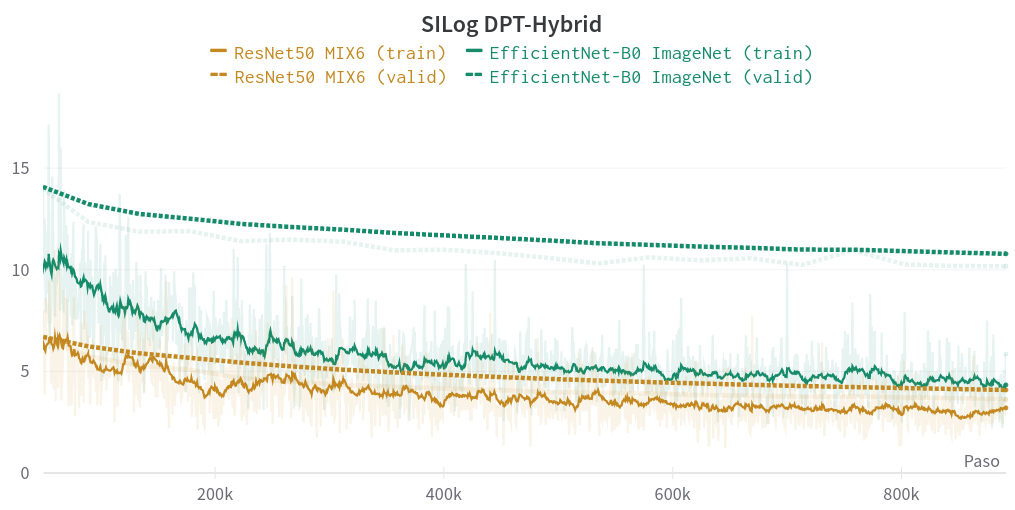
\includegraphics[width=0.95\linewidth]{imagenes/Resultados/EfficientNet_overfitting.png} 
\captionsetup{width=.95\linewidth}
\caption{Comparación de las curvas de aprendizaje del SIlog durante el entrenamiento y validación de dos modelos con diferentes \textit{backbones} e inicializaciones de pesos. Valores suavizados con una media exponencial ponderada para facilitar su visualización.}
\label{fig:efficientnet-overfitting}
\end{figure}

Dado que los parámetros de EfficientNet-B0 se han inicializado con parámetros entrenados en ImageNet y no en MIX6 (\textit{dataset} de profundidad utilizado para preentrenar las ResNet50), se plantea un experimento adicional para descartar que esta falta de preentrenamiento especializado sea la causa del \textit{overfitting}. Para llevar a cabo este experimento, se extraen los parámetros de un ViT-Hybrid preentrenado en ImageNet y se utilizan para inicializar los pesos de un DPT-Hybrid con ResNet50. De esta forma, la ResNet50 parte de un estado similar al de la EfficientNet-B0 (preentrenamiento en ImageNet). En la \Cref{fig:mix6-imagenet}, se pueden apreciar los resultados en el conjunto de validación de estos tres modelos y se comprueba como el dominio del preentrenamiento no influye en el sobreajuste del \textit{backbone} convolucional.

\begin{figure}[H]
\centering
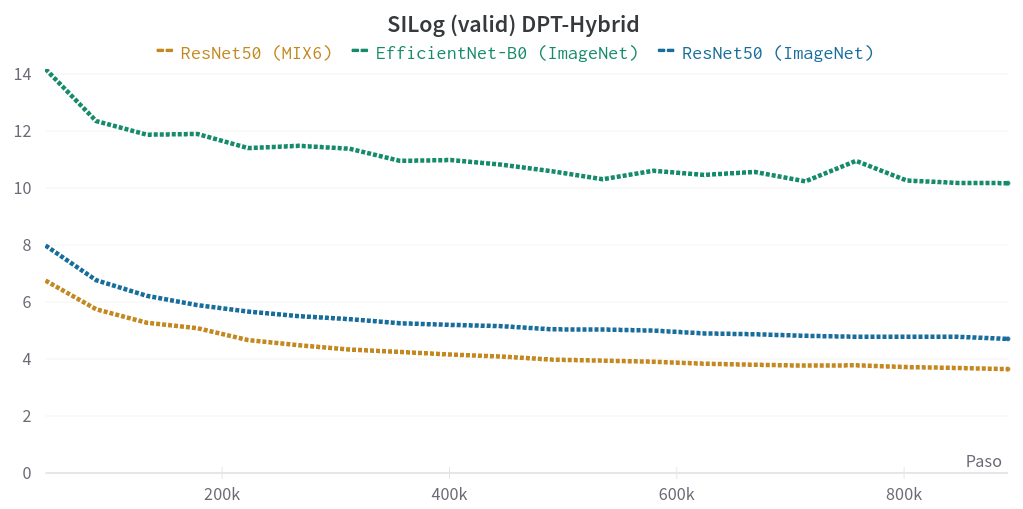
\includegraphics[width=0.95\linewidth]{imagenes/Resultados/ResNet50ImageNet.png} 
\captionsetup{width=.95\linewidth}
\caption{Comparación del SIlog en el conjunto de validación durante el entrenamiento en tres modelos con diferentes inicializaciones de pesos.}
\label{fig:mix6-imagenet}
\end{figure}














































\subsection{Número de cabezas}\label{resultados-cuantitativos-cabezas}

En la \Cref{fig:SIlog-val-split}, equivalente a la \Cref{fig:SIlog-validation} pero separada en función del \textit{backbone}, es posible ver como la diferencia en los resultados según el número de cabezas en los bloques de atención es relativamente pequeña, especialmente en el caso del mecanismo de atención estándar.

\begin{figure}[H]
\centering
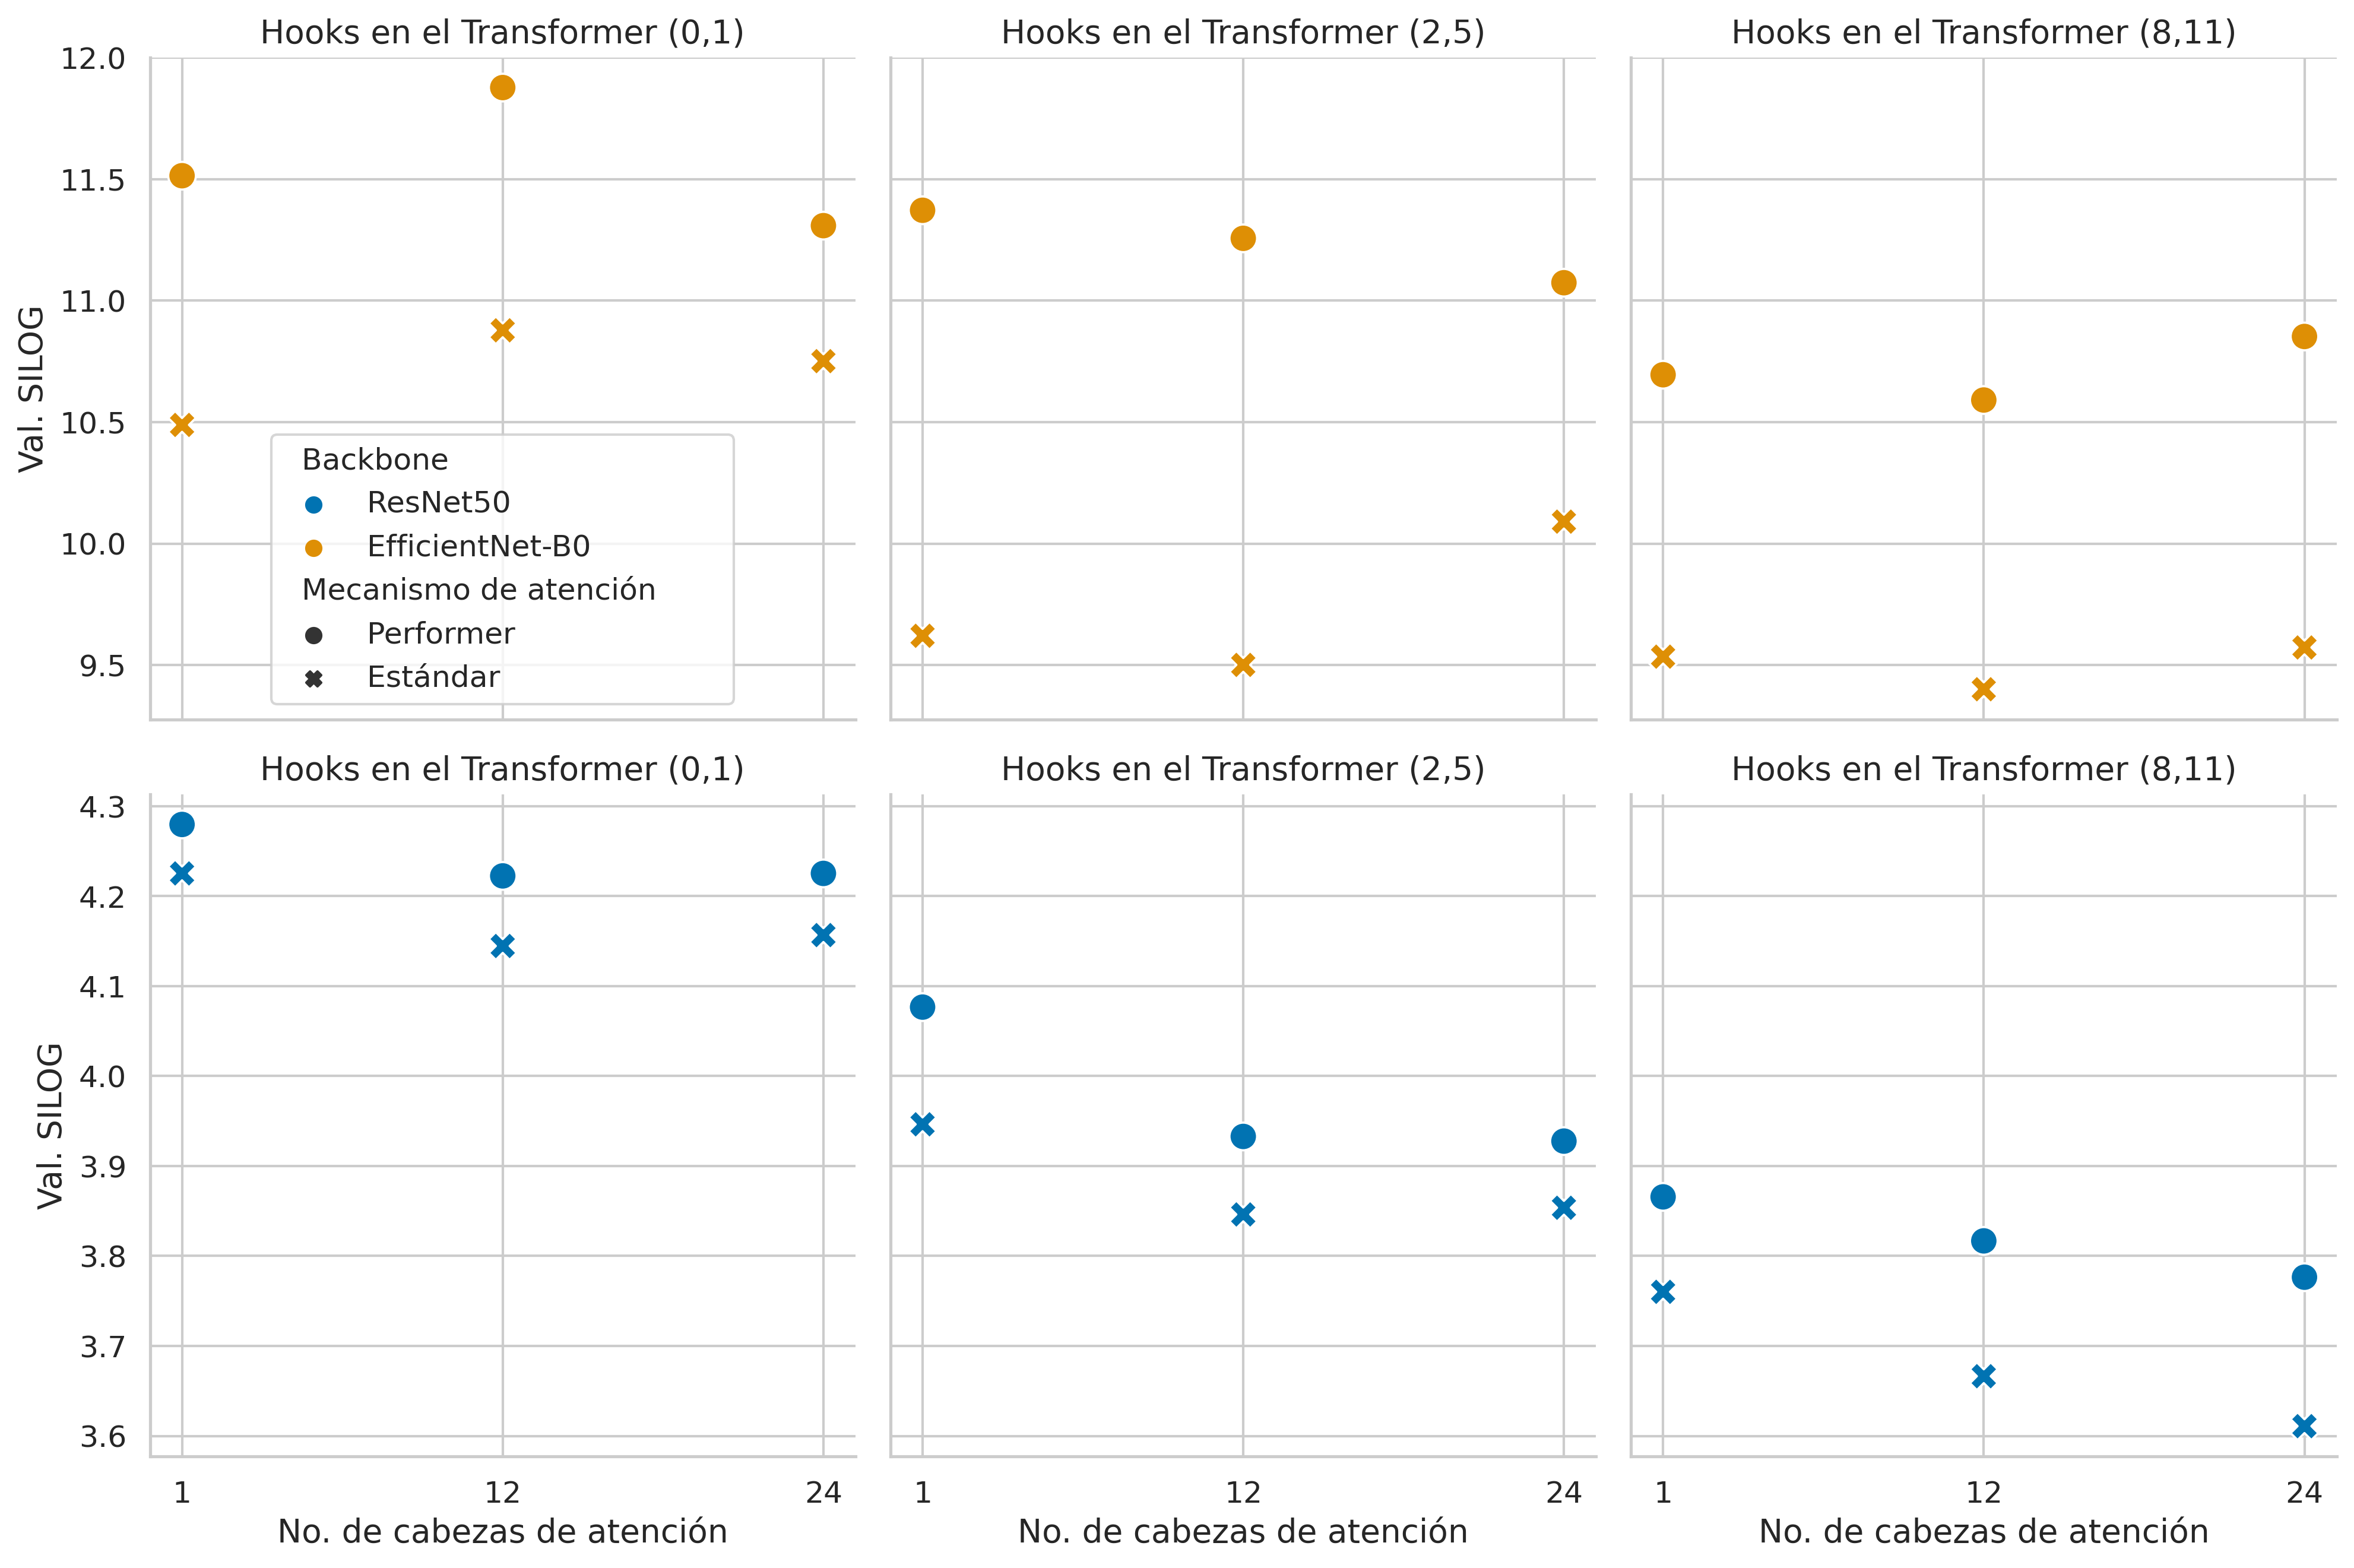
\includegraphics[width=\linewidth]{imagenes/Resultados/SIlog_val_split.png} 
\captionsetup{width=.95\linewidth}
\caption{SIlog obtenido en el conjunto de validación para cada uno de los 36 modelos entrenados con distintos ejes en función del \textit{backbone}. Más bajo es mejor.}
\label{fig:SIlog-val-split}
\end{figure}

De forma similar, en el caso de las métricas de velocidad de inferencia (\Cref{fig:resultados-inf-num-cabezas}), sobretodo en el caso de las imágenes reducidas, no se encuentra un aumento de la velocidad especialmente significativo.

\begin{figure}[H]
\centering
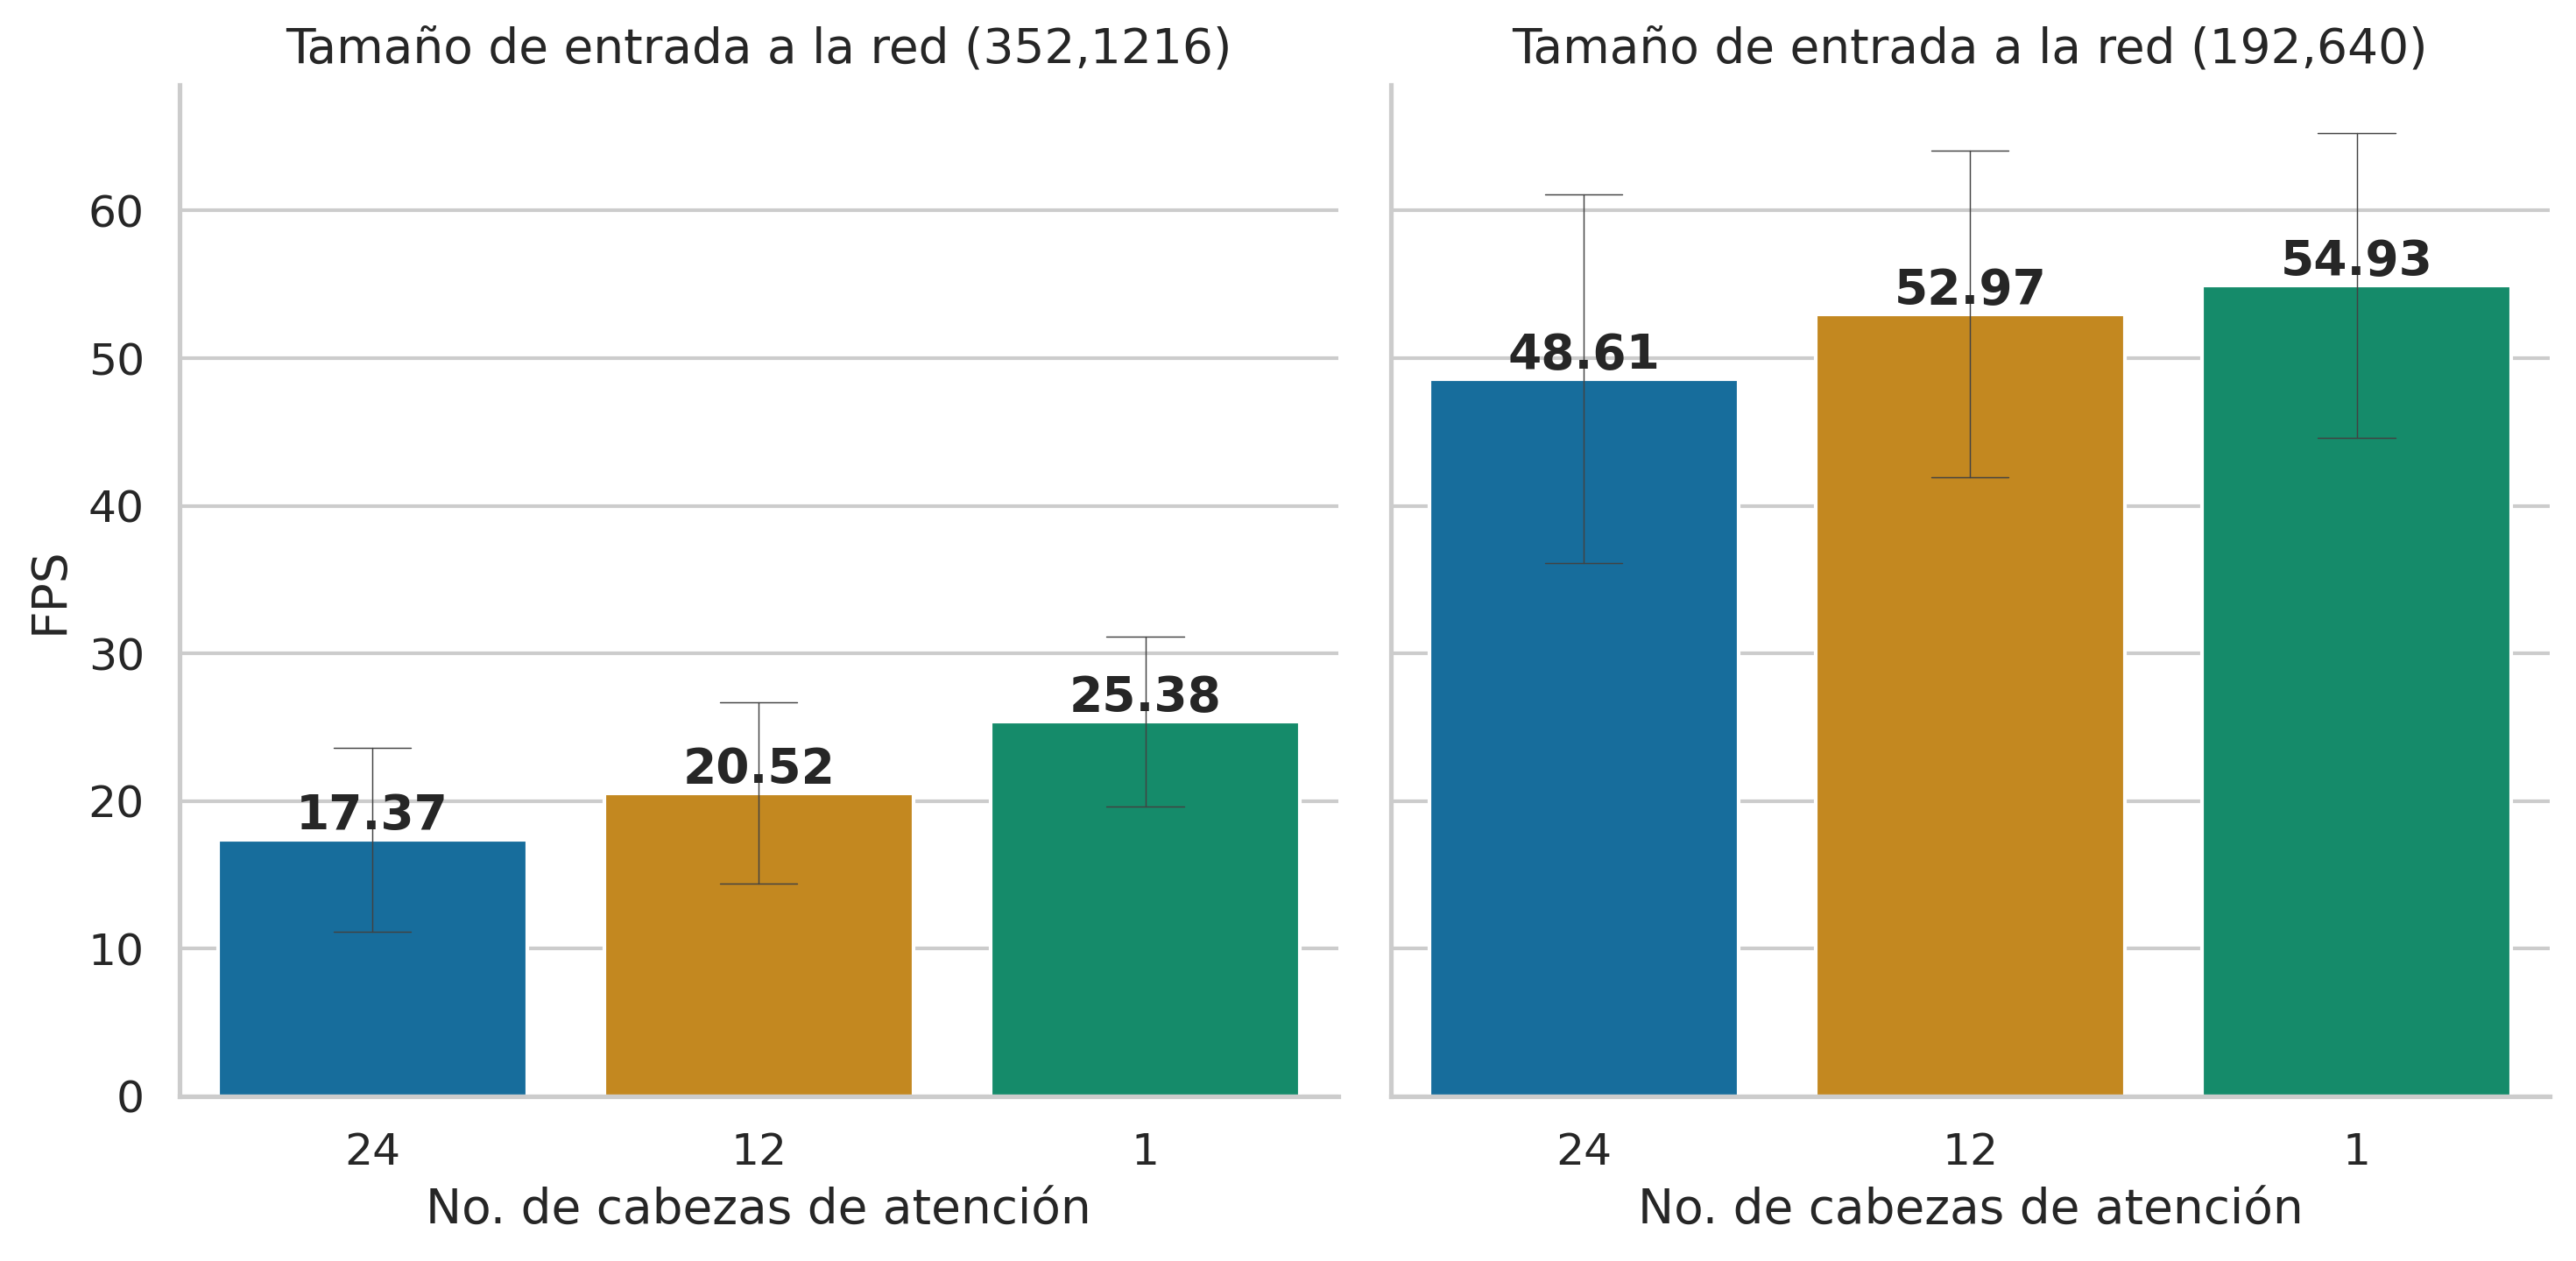
\includegraphics[width=0.75\linewidth]{imagenes/Resultados/velocidad_inferencia_cabezas_atencion.png} 
\captionsetup{width=.8\linewidth}
\caption{FPS medios de los modelos en función del número de cabezas utilizado y del tamaño de la entrada. Las barras grises representan la desviación estándar de las medidas.}
\label{fig:resultados-inf-num-cabezas}
\end{figure}
























\subsection{Capas de atención eficiente}\label{resultados-cuantitativos-atencion}
Tal y como se ha visto en la \Cref{fig:SIlog-val-split}, el cambio del mecanismo de atención eficiente también influye negativamente en la calidad de los resultados. Dado que el incremento de la métrica de error es relativamente pequeño, esto podría ser totalmente aceptable si no fuese por los resultados de las métricas de velocidad (\Cref{fig:resultados-inf-mec-atention}), donde se puede observar que los modelos con el mecanismo de atención eficiente (\textit{Performer}) son en realidad más lentos cuando el tamaño de la entrada es reducido.

\begin{figure}[H]
\centering
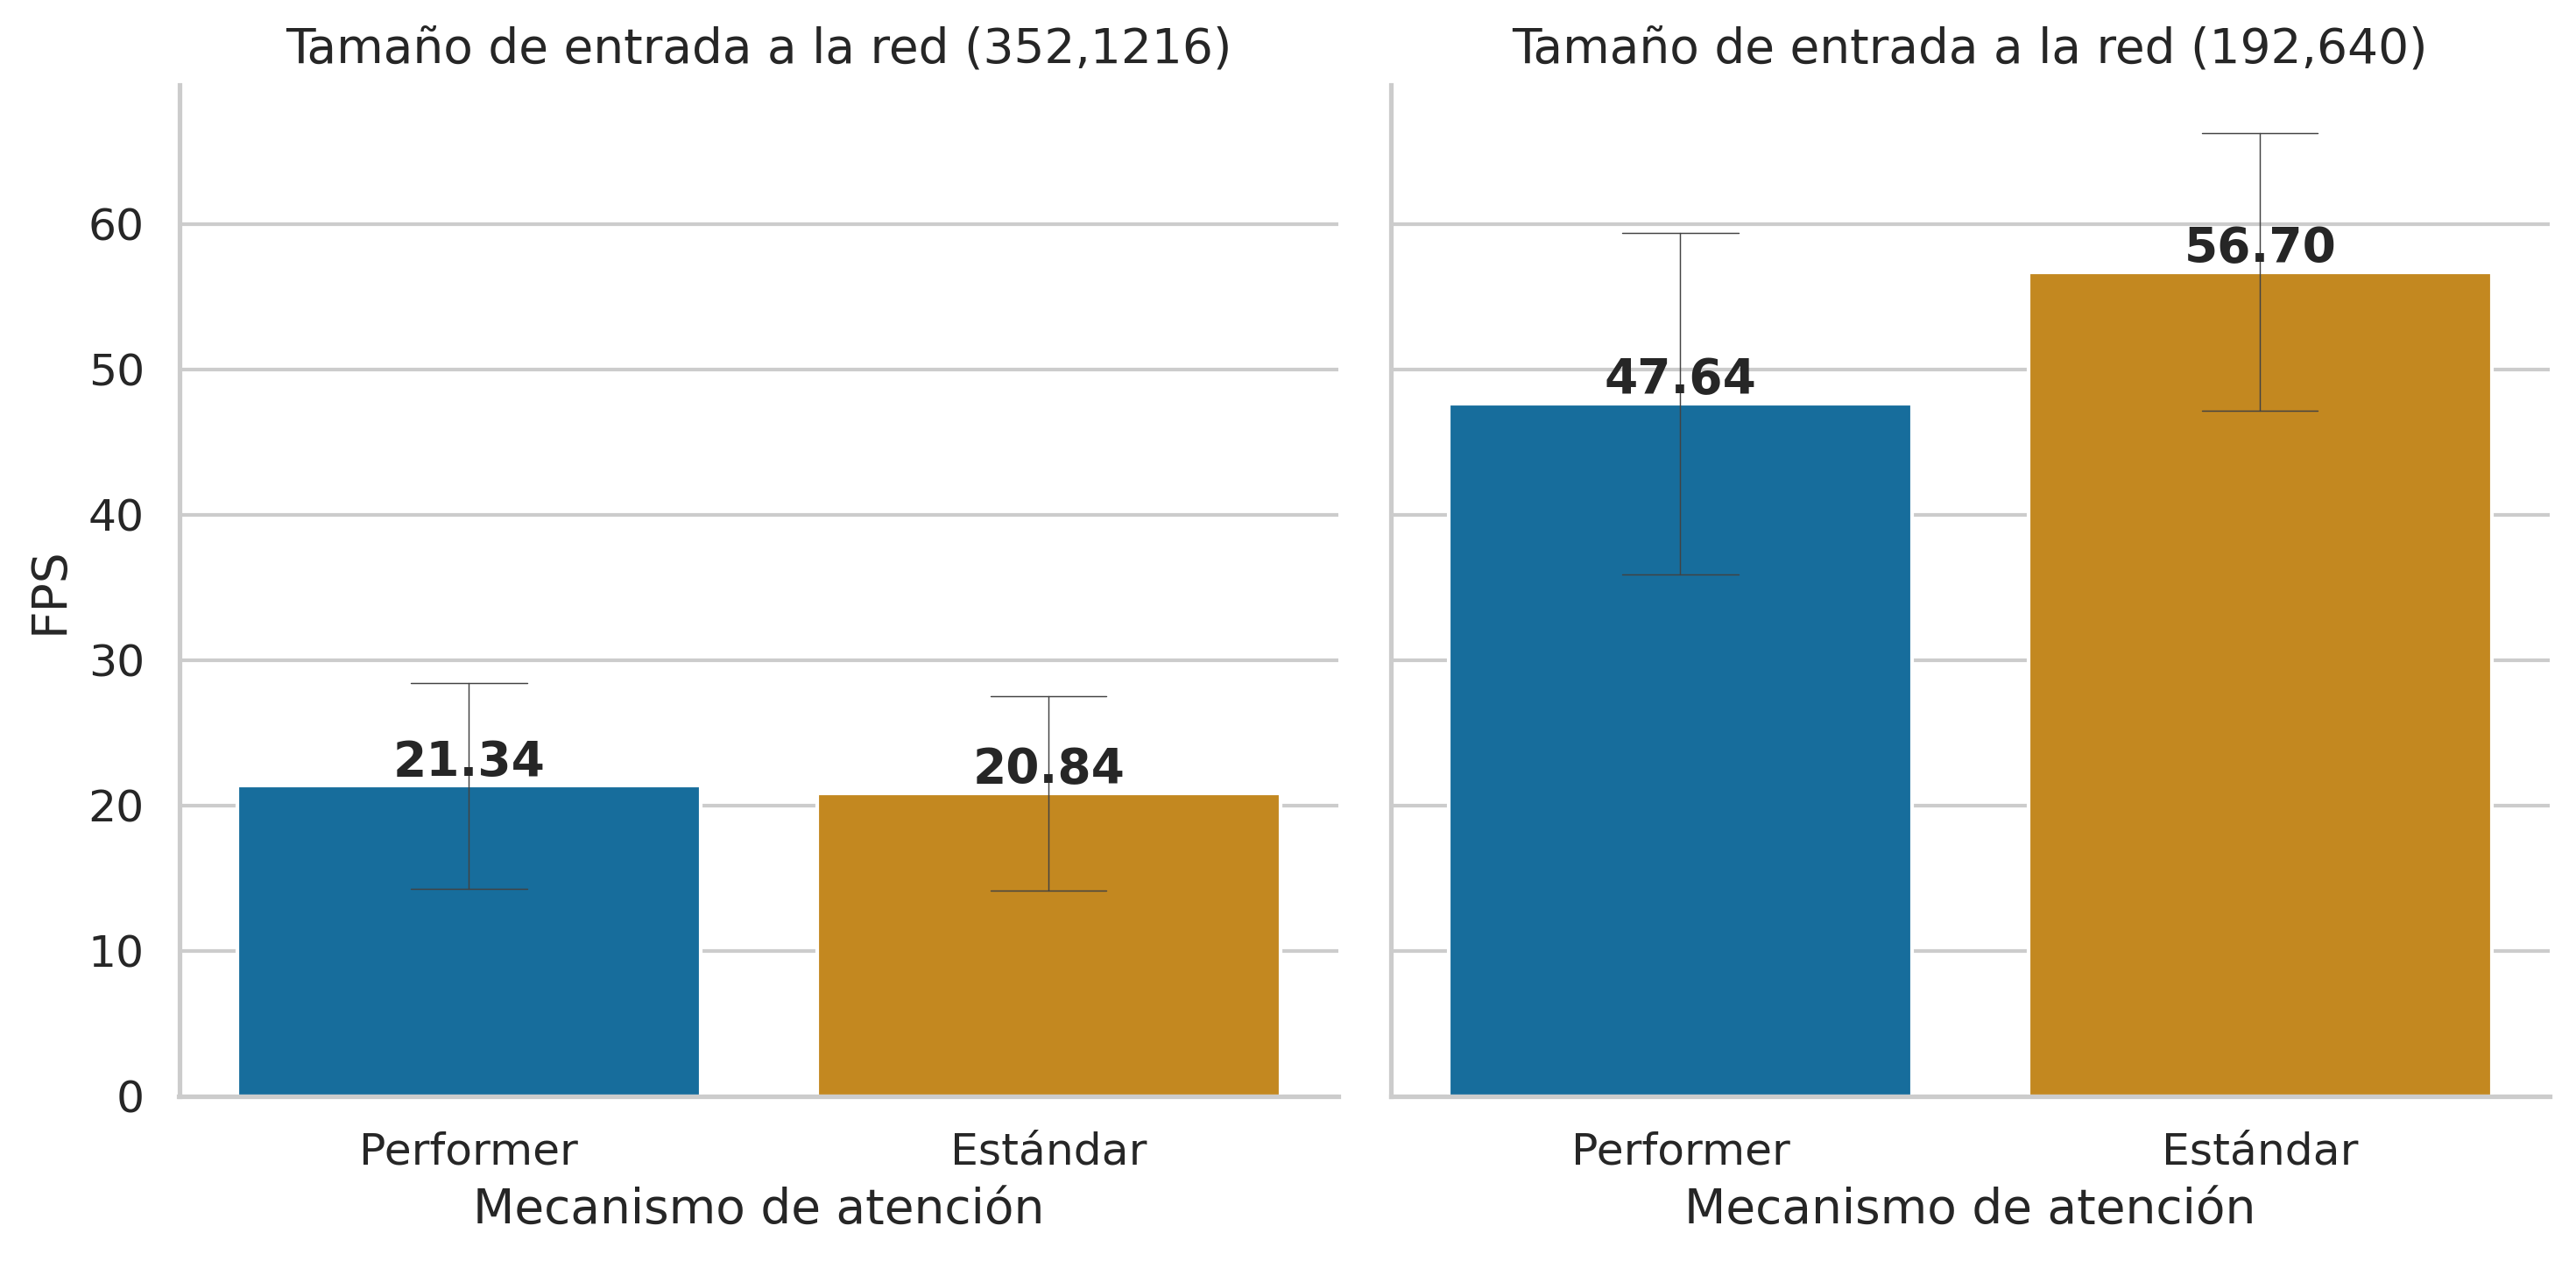
\includegraphics[width=0.9\linewidth]{imagenes/Resultados/velocidad_inferencia_mecanismo_atencion.png} 
\captionsetup{width=.9\linewidth}
\caption{FPS medios de los modelos en función del mecanismo de atención utilizado y del tamaño de la entrada. Las barras grises representan la desviación estándar de las medidas.}
\label{fig:resultados-inf-mec-atention}
\end{figure}

Esto, se debe a que, pese a que la complejidad del mecanismo de atención eficiente es $O(n)$ y la del mecanismo de atención estándar es $O(n^2)$, existe un \textit{overhead} asociado al mecanismo de atención eficiente que hace que la ejecución para secuencia de elementos cortas (como es el caso de la imagen reducida) sea más lento que con la atención estándar. En la \Cref{fig:resultados-complejidad-mec-atencion}, donde se muestran los resultados de otro experimento donde se incrementó la longitud de la secuencia de entrada progresivamente para medir el tiempo de inferencia de un bloque de atención, se puede apreciar este comportamiento.

\begin{figure}[H]
\centering
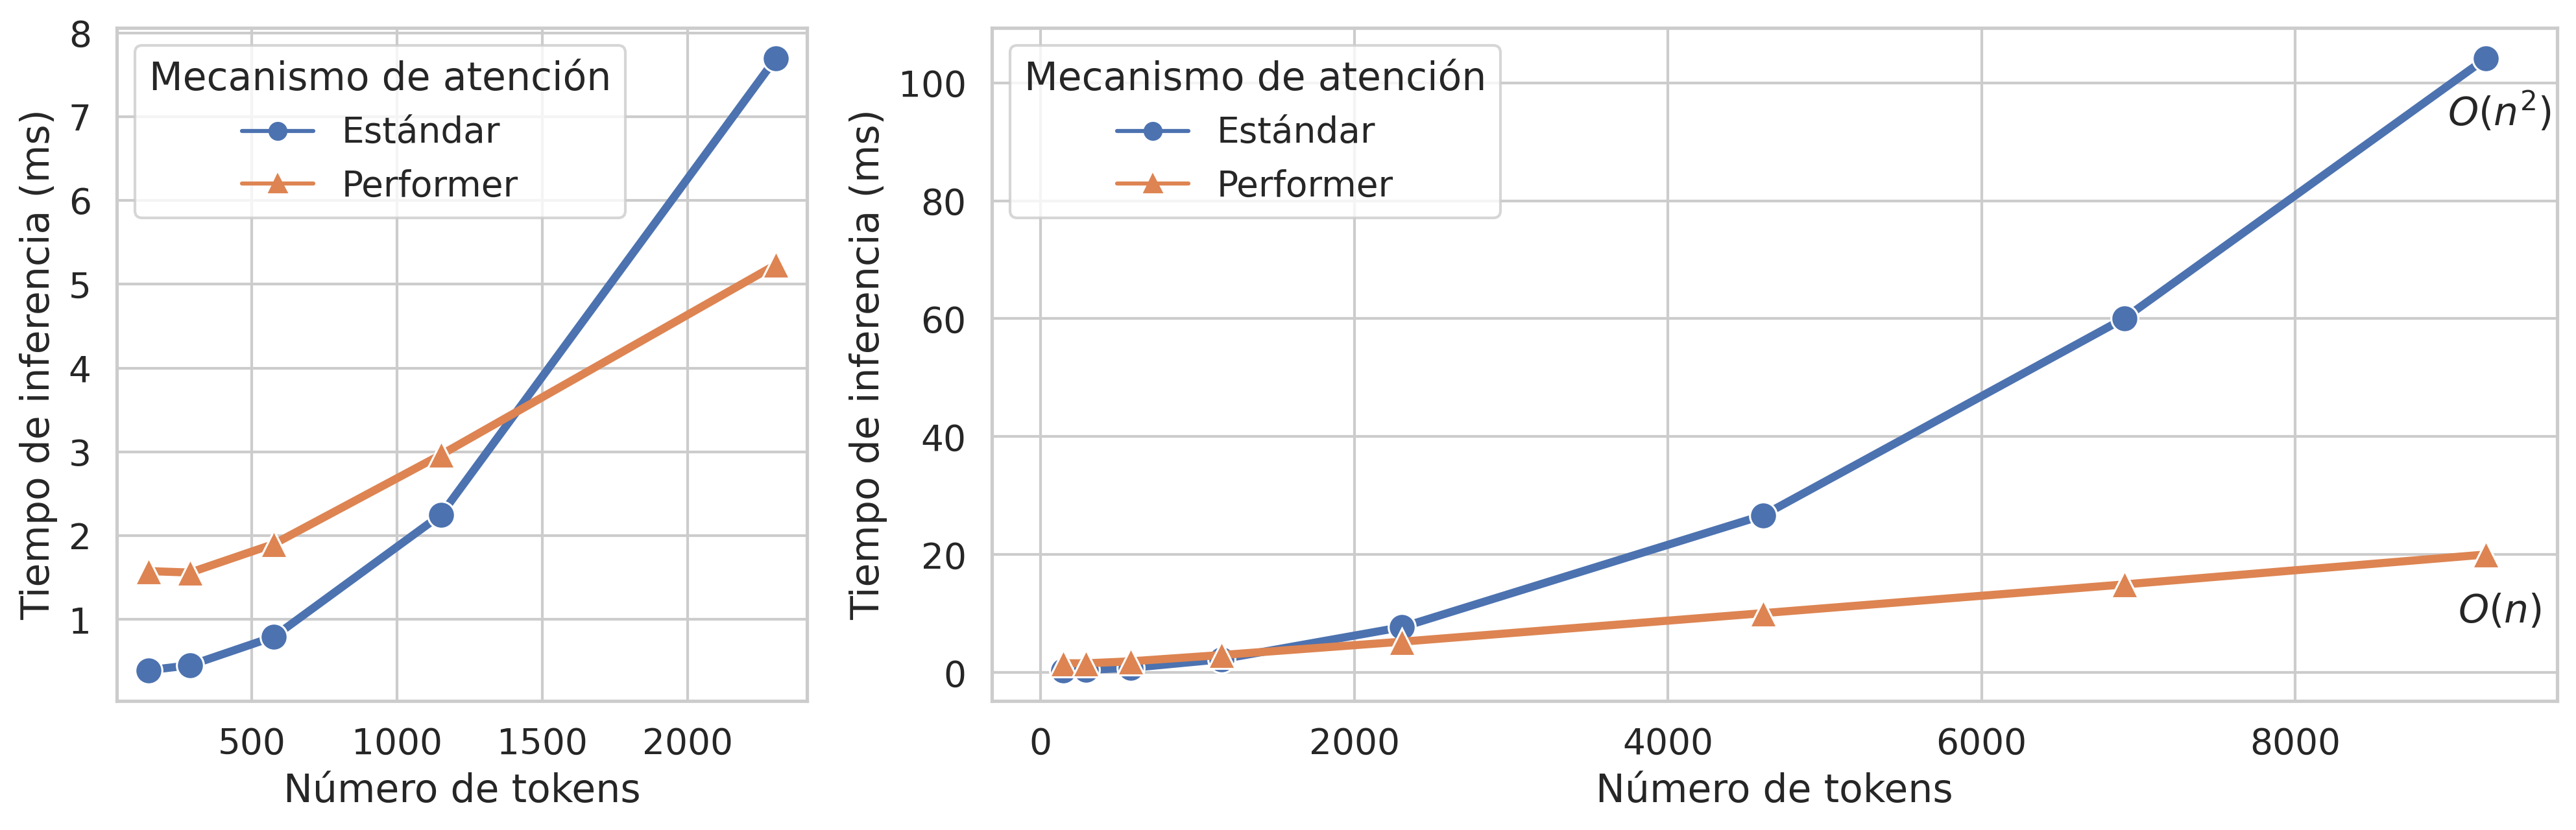
\includegraphics[width=\linewidth]{imagenes/Resultados/complejidad_mecanismo_atencion.png} 
\captionsetup{width=.95\linewidth}
\caption{Comparación de la complejidad y el tiempo de inferencia en un bloque de atención usando el mecanismo de atención estándar y el mecanismo eficiente del \textit{Performer}. Detalle de los tiempos de inferencia para entradas con un número de \textit{tokens} reducido a la izquierda.}
\label{fig:resultados-complejidad-mec-atencion}
\end{figure}

















\subsection{Cambio en los hooks del transformer y eliminación de las capas de atención posteriores}\label{resultados-cuantitativos-hooks}
La última modificación de la arquitectura estudiada, el cambio en los \textit{hooks}, es decir, la elección de los bloques de atención de los cuales se toman las salidas como entradas del \textit{encoder} es, después del cambio de \textit{backbone}, la que más afecta a la calidad de los resultados (\Cref{fig:SIlog-val-split}). Por otro lado, el incremento en la velocidad de inferencia asociado a este cambio sí que es considerable (\Cref{fig:resultados-inf-hooks}) llegando casi a duplicar los FPS en los modelos con la entrada a resolución original y aumentando en más de un $50\%$ los FPS cuando el tamaño de la entrada se ha reducido.

\begin{figure}[H]
\centering
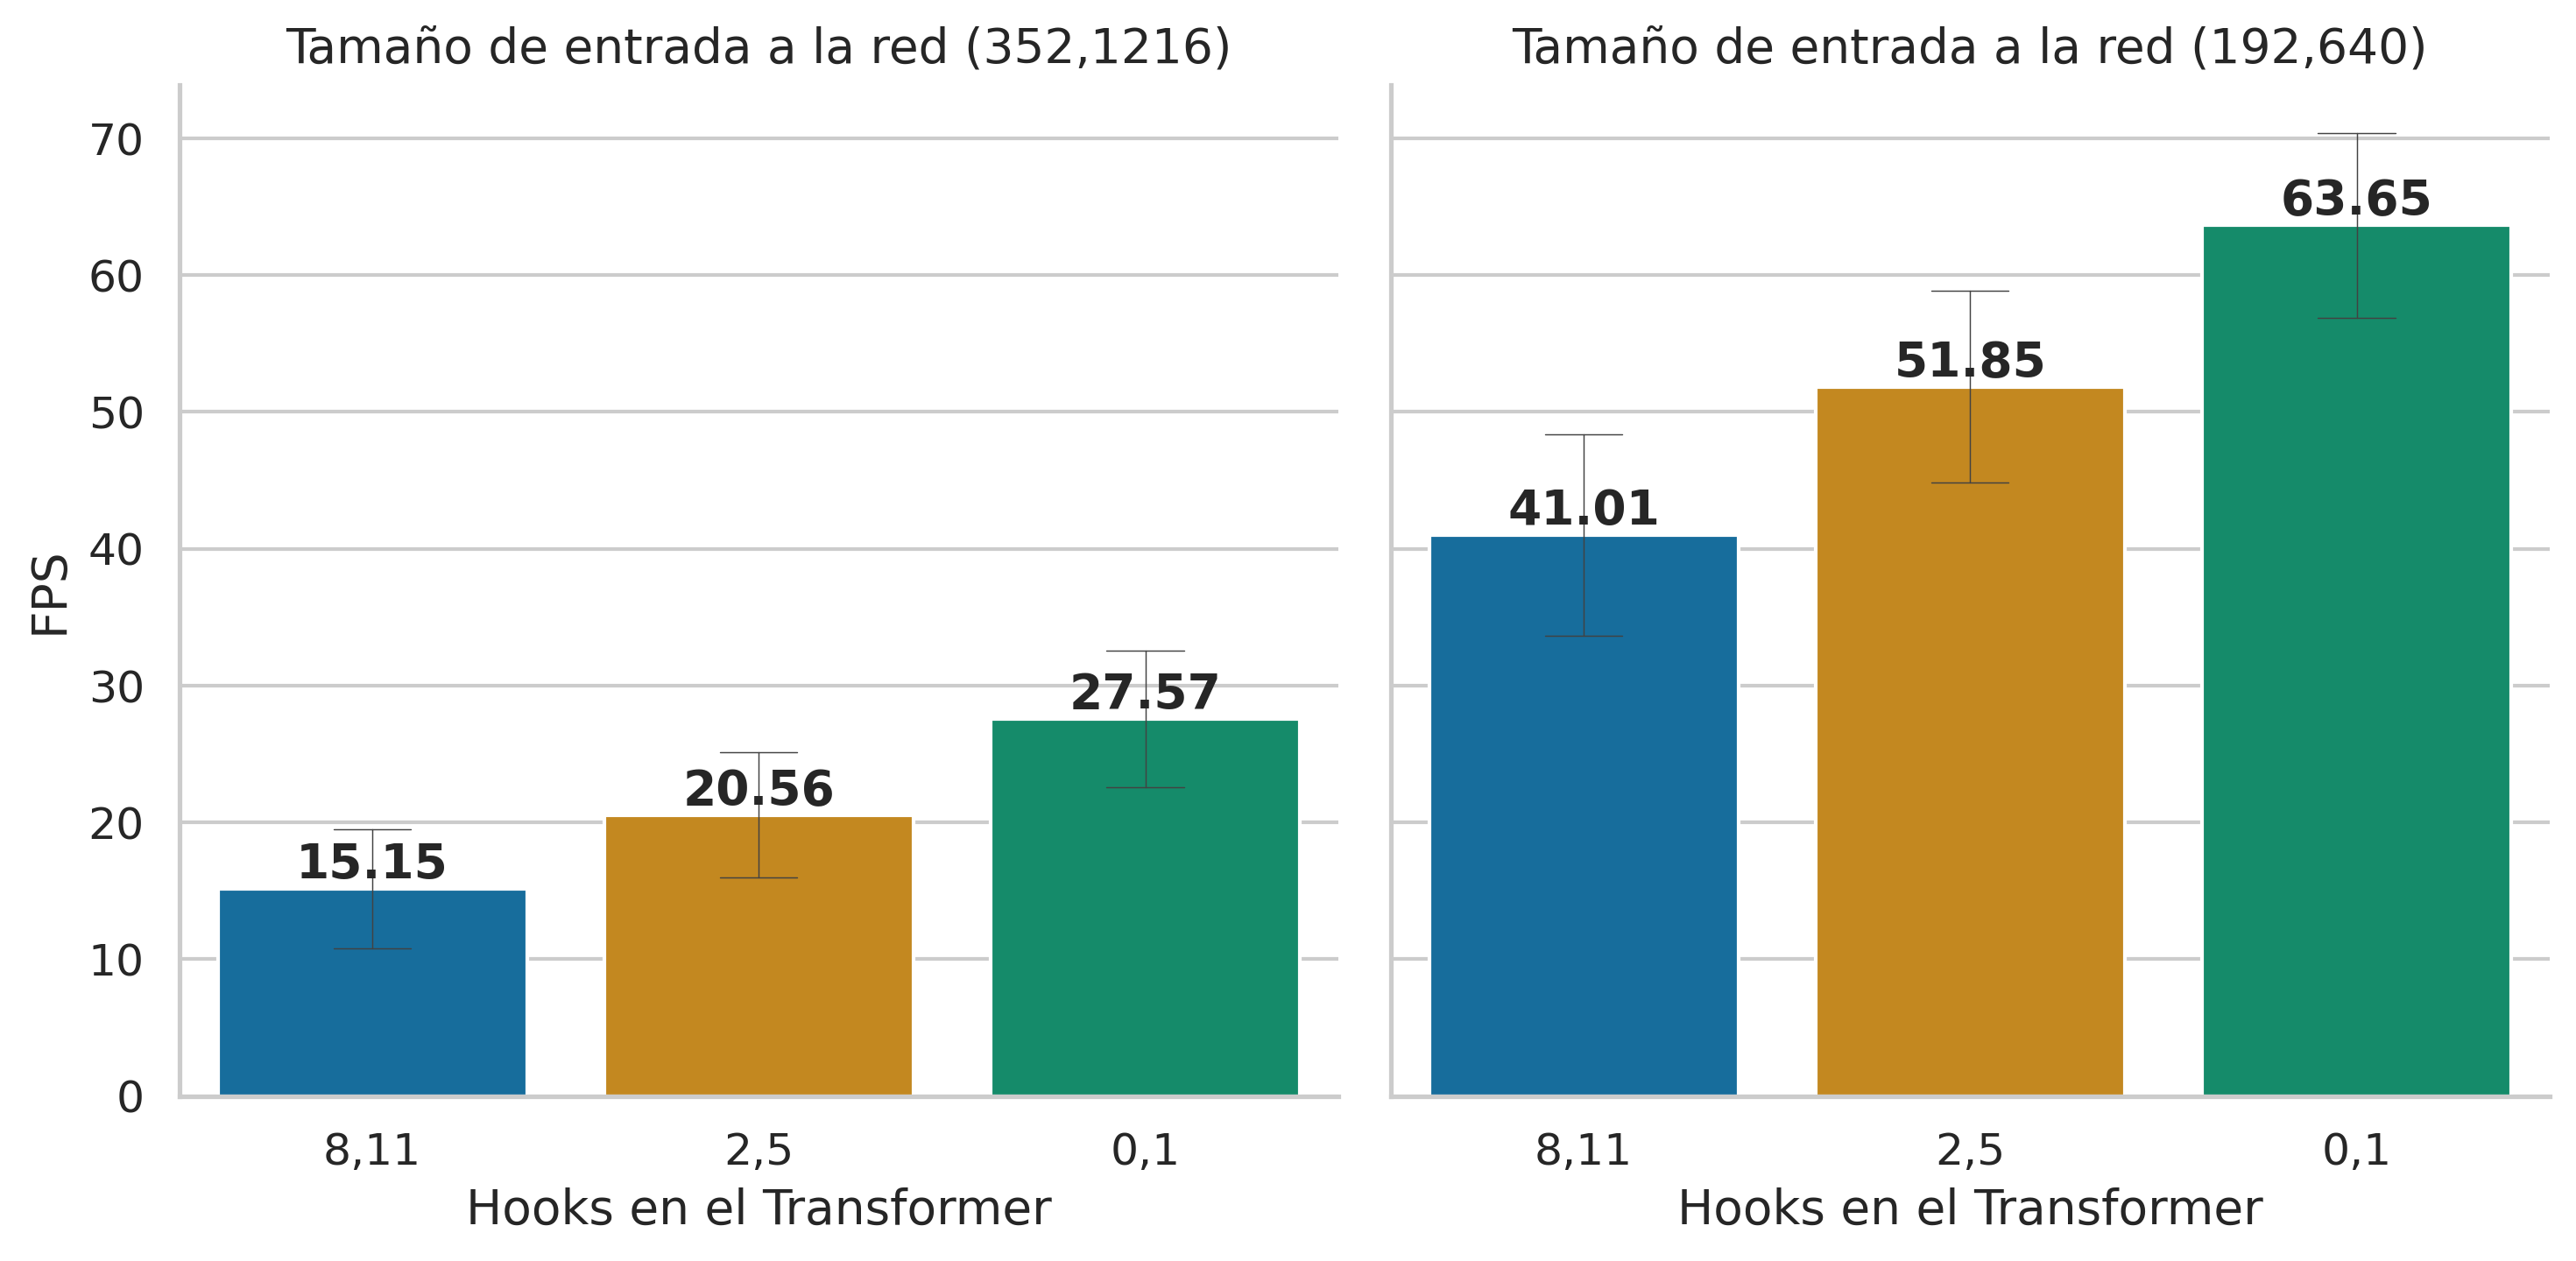
\includegraphics[width=0.85\linewidth]{imagenes/Resultados/velocidad_inferencia_hooks.png} 
\captionsetup{width=.9\linewidth}
\caption{FPS medios de los modelos en función de los \textit{hooks} utilizados y del tamaño de la entrada. Las barras grises representan la desviación estándar de las medidas.}
\label{fig:resultados-inf-hooks}
\end{figure}















\section{Tamaño de los modelos y número de operaciones}
El tamaño de los modelos también se ve afectado por las modificaciones del modelo que se han llevado a cabo en este proyecto. En la \Cref{fig:resultados-mb} se puede ver el tamaño en \textit{megabytes} (MB) que ocupan los modelos. En esta gráfica, puede apreciarse como la mayor diferencia viene dada por los bloques donde se situan los \textit{hooks} ya que al elegir los bloques iniciales del \textit{transformer} es posible eliminar todos los parámetros correspondientes a los bloques de atención posteriores. Cabe destacar también de estos resultados cómo la diferencia de tamaño entre los modelos en función del \textit{backbone} convolucional es relativamente pequeña, y la forma en que el número de cabezas afecta al tamaño del modelo en función del mecanismo de atención empleado.


\begin{figure}[H]
\centering
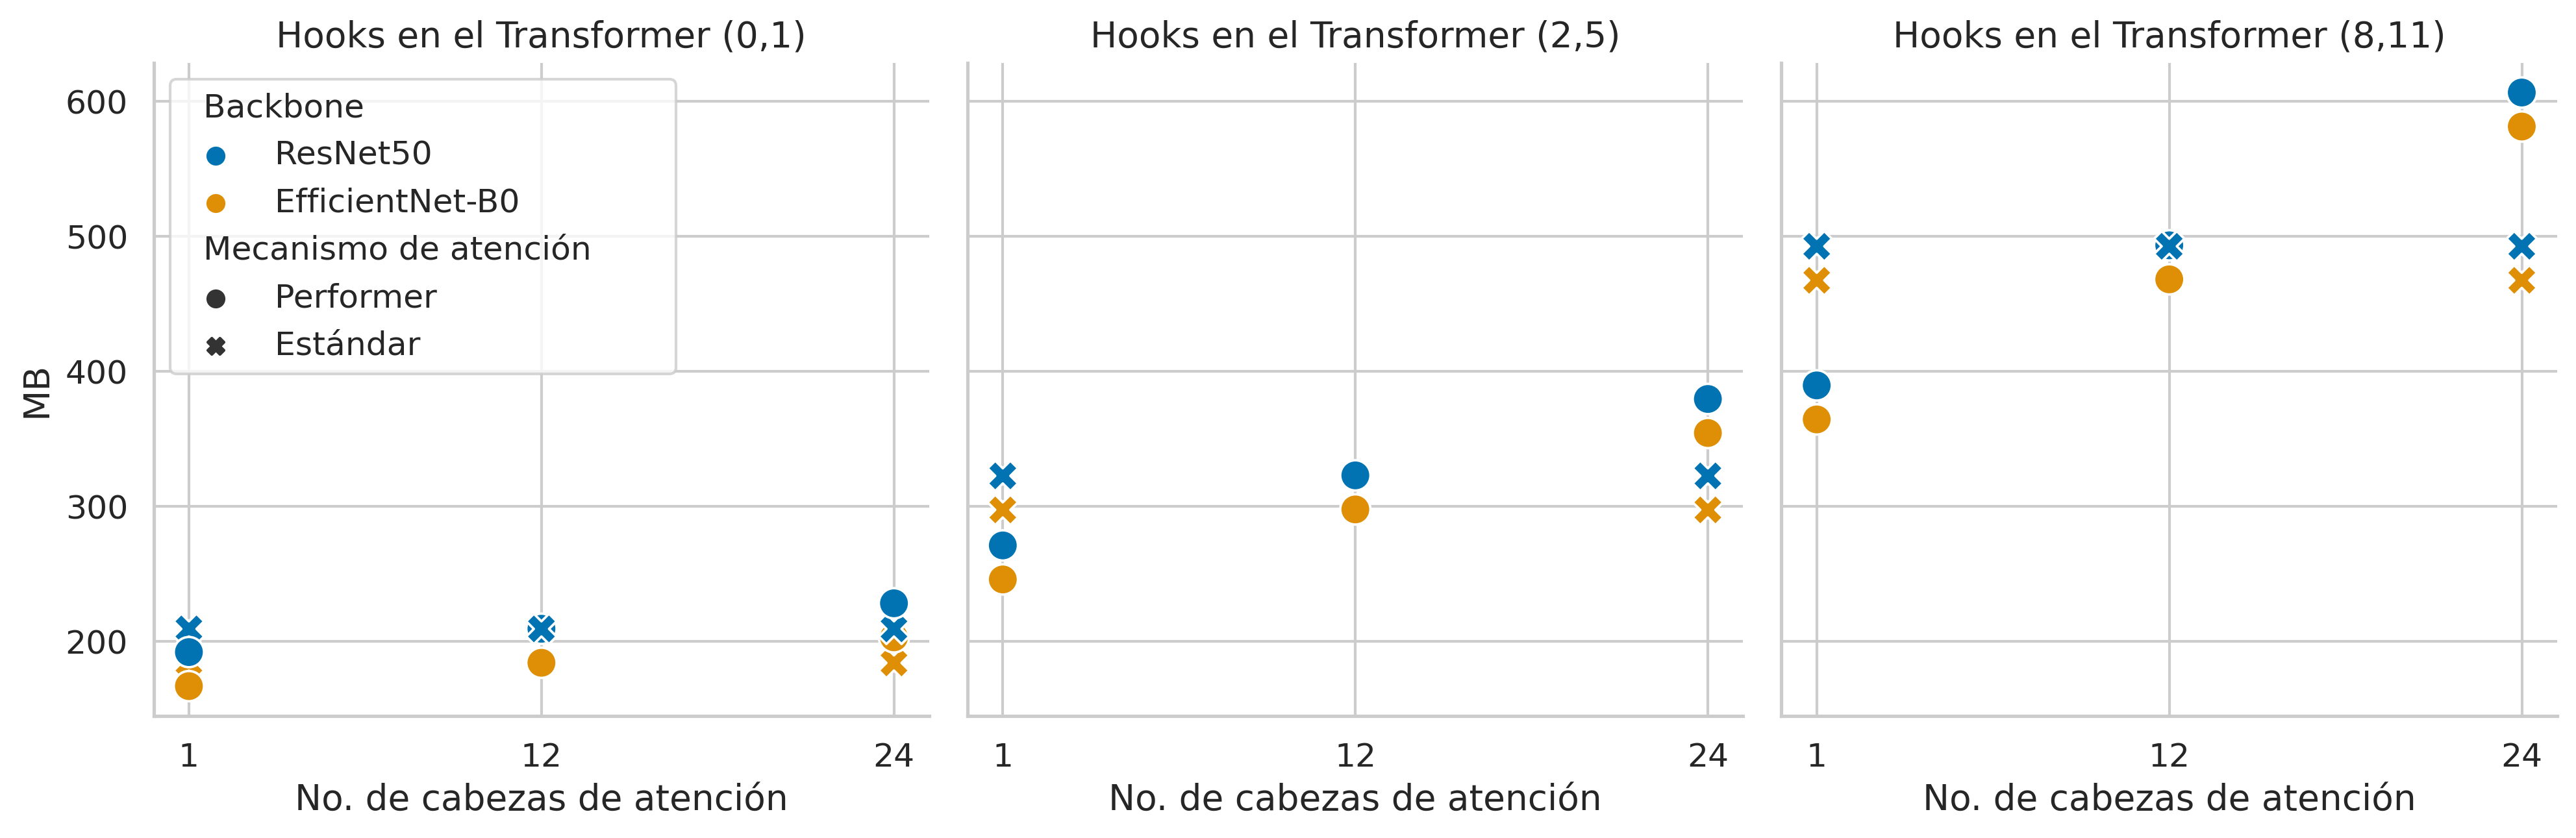
\includegraphics[width=\linewidth]{imagenes/Resultados/mb.png} 
\captionsetup{width=0.95\linewidth}
\caption{Tamaño en memoria de los modelos en función de su configuración.}
\label{fig:resultados-mb}
\end{figure}

La tendencia de los tamaños de los modelos en función de sus características es posible verla también en las medidas de Giga FLOPs (número de operaciones en coma flotante requeridas para inferir la salida con una sola entrada) presentadas en la \Cref{fig:resultados-gflops}. No obstante, una diferencia interesante entre estas dos Figuras es que en el número de operaciones necesarias para obtener la salida del modelo sí que influye en mayor medida la elección del \textit{backbone} convolucional, es decir, se puede comprobar que para un número de parámetros similar, EfficientNet-B0 lleva a cabo un número de operaciones menor que ResNet50.

\begin{figure}[H]
\centering
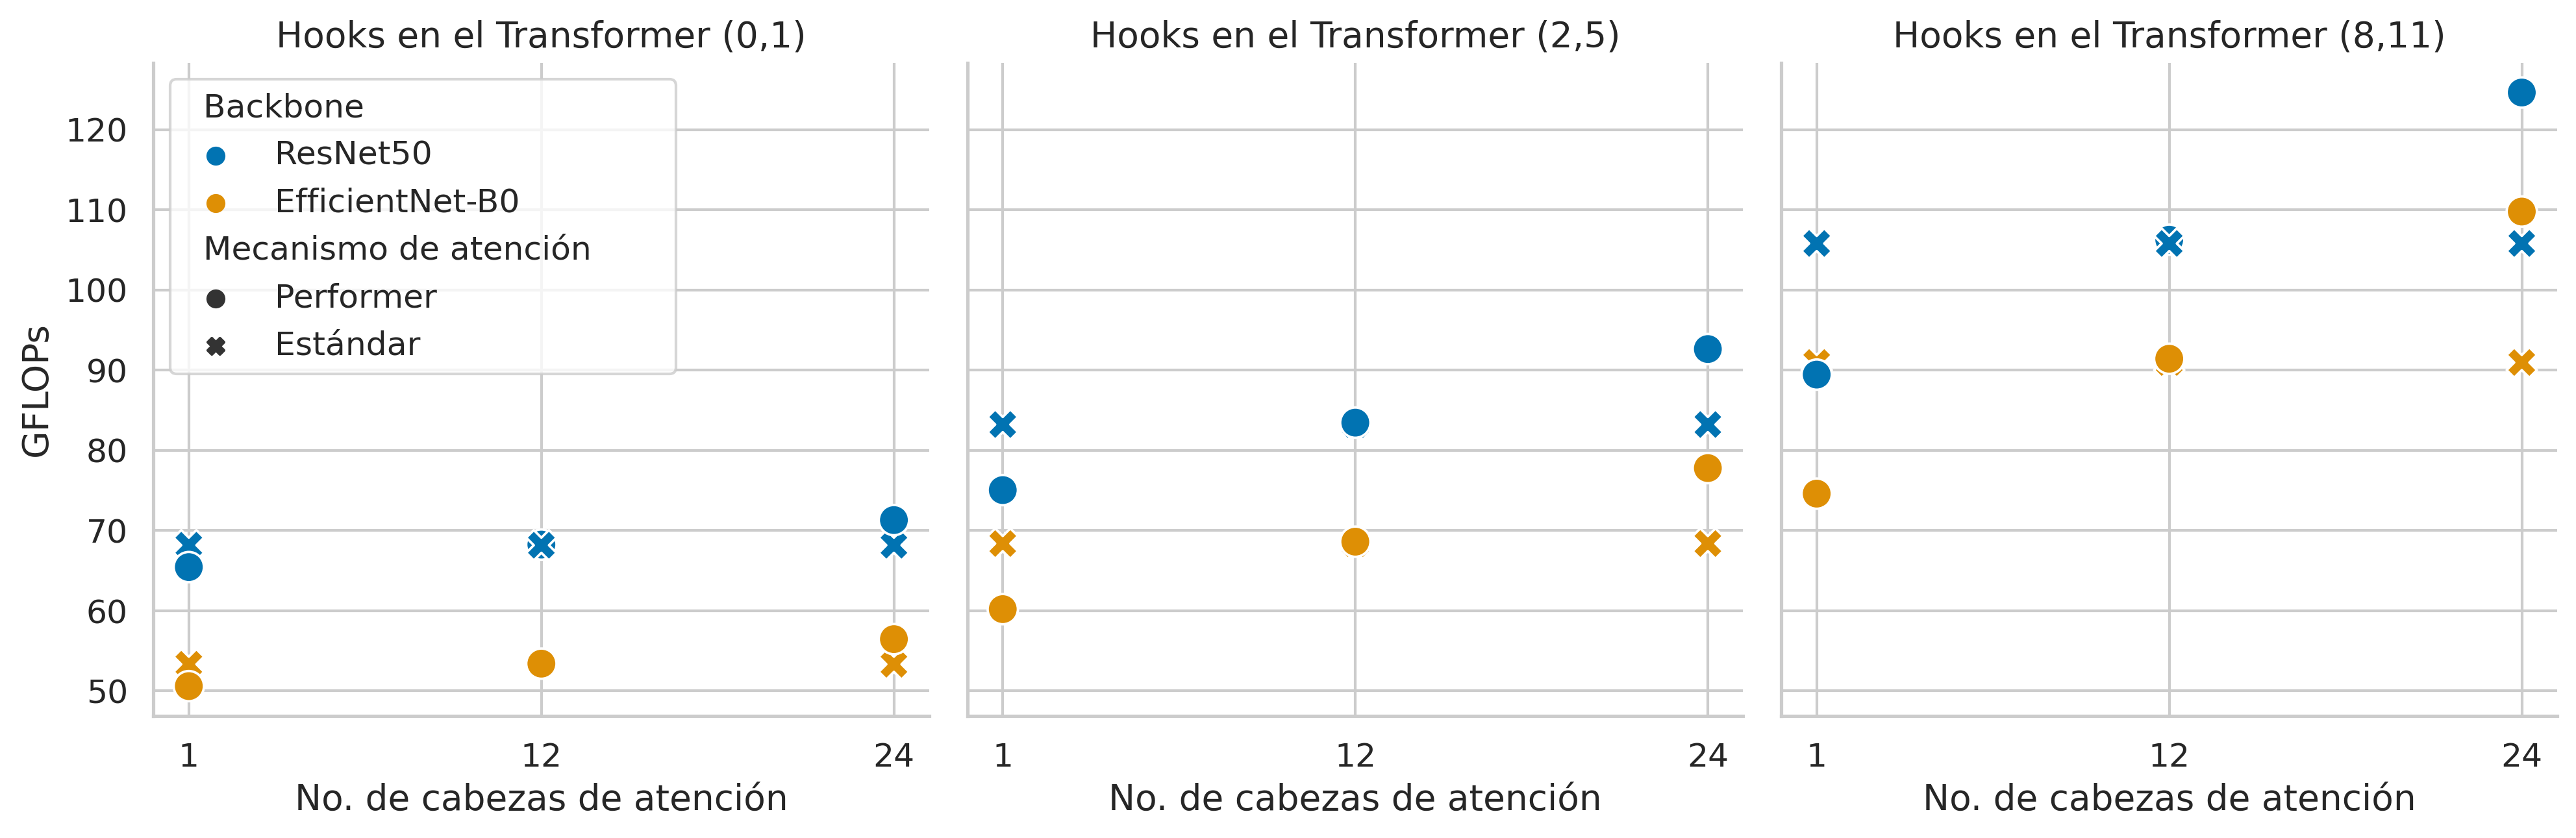
\includegraphics[width=\linewidth]{imagenes/Resultados/gflops.png} 
\captionsetup{width=.95\linewidth}
\caption{Número de operaciones en coma flotante necesarias para inferir la profundidad en una imagen en función de la configuración del modelo.}
\label{fig:resultados-gflops}
\end{figure}













\pagebreak

\section{Resultados cualitativos}

En esta sección, se presentan los resultados en el conjunto de evaluación (\textit{test}) de distintos modelos en función de sus modificaciones, con el objetivo de comparar visualmente y apreciar las diferencias entre las salidas que generan las distintas arquitecturas. Los valores de las imágenes generadas por el modelo solamente ocupan una pequeña parte de la escala de grises, por lo tanto, para facilitar la apreciación de detalles, las imágenes mostradas a continuación han sido previamente normalizadas de forma que ocupen todo el rango de grises. 

%% http://www.peteryu.ca/tutorials/publishing/latex_captions_old
%% https://tex.stackexchange.com/questions/162824/vertical-spacing-between-subfloat
%% https://tex.stackexchange.com/questions/395515/how-to-scale-and-align-figures-and-tables-in-latex-in-a-3x2-grid-like-manner




%\captionsetup[subfigure]{labelformat=empty}
%    \begin{figure}[!ht]
%\centering
%    \subfloat{\includegraphics[width=0.33\linewidth]{imagenes/test_output_samples/input/2011_09_26_drive_0002_sync_0000000021.png}}
%\hfil
%    \subfloat{\includegraphics[width=0.33\linewidth]{imagenes/test_output_samples/2011_09_26_drive_0002_sync_0000000021/e7069aae.png}}
%\hfil
%    \subfloat{\includegraphics[width=0.33\linewidth]{imagenes/test_output_samples/2011_09_26_drive_0002_sync_0000000021/qsudwuyk.png}}\\[-2ex]
%
%
%    \subfloat{\includegraphics[width=0.33\linewidth]{imagenes/test_output_samples/input/2011_09_26_drive_0009_sync_0000000112.png}}
%\hfil
%    \subfloat{\includegraphics[width=0.33\linewidth]{imagenes/test_output_samples/2011_09_26_drive_0009_sync_0000000112/e7069aae.png}}
%\hfil
%    \subfloat{\includegraphics[width=0.33\linewidth]{imagenes/test_output_samples/2011_09_26_drive_0009_sync_0000000112/qsudwuyk.png}}\\[-2ex]
%    
%    
%    \subfloat{\includegraphics[width=0.33\linewidth]{imagenes/test_output_samples/input/2011_09_26_drive_0009_sync_0000000196.png}}
%\hfil
%    \subfloat{\includegraphics[width=0.33\linewidth]{imagenes/test_output_samples/2011_09_26_drive_0009_sync_0000000196/e7069aae.png}}
%\hfil
%    \subfloat{\includegraphics[width=0.33\linewidth]{imagenes/test_output_samples/2011_09_26_drive_0009_sync_0000000196/qsudwuyk.png}}\\[-2ex]
%    
%    
%    
%    \subfloat{\includegraphics[width=0.33\linewidth]{imagenes/test_output_samples/input/2011_09_26_drive_0009_sync_0000000292.png}}
%\hfil
%    \subfloat{\includegraphics[width=0.33\linewidth]{imagenes/test_output_samples/2011_09_26_drive_0009_sync_0000000292/e7069aae.png}}
%\hfil
%    \subfloat{\includegraphics[width=0.33\linewidth]{imagenes/test_output_samples/2011_09_26_drive_0009_sync_0000000292/qsudwuyk.png}}\\[-2ex]
%    
%    
%    
%    \subfloat{\includegraphics[width=0.33\linewidth]{imagenes/test_output_samples/input/2011_09_26_drive_0009_sync_0000000324.png}}
%\hfil
%    \subfloat{\includegraphics[width=0.33\linewidth]{imagenes/test_output_samples/2011_09_26_drive_0009_sync_0000000324/e7069aae.png}}
%\hfil
%    \subfloat{\includegraphics[width=0.33\linewidth]{imagenes/test_output_samples/2011_09_26_drive_0009_sync_0000000324/qsudwuyk.png}}\\[-2ex]
%
%
%
%    \subfloat[Entrada]{\includegraphics[width=0.33\linewidth]{imagenes/test_output_samples/input/2011_09_26_drive_0013_sync_0000000030.png}}
%\hfil
%    \subfloat[Salida DPT sin modificar]{\includegraphics[width=0.33\linewidth]{imagenes/test_output_samples/2011_09_26_drive_0013_sync_0000000030/e7069aae.png}}
%\hfil
%    \subfloat[Salida DPT modificado]{\includegraphics[width=0.33\linewidth]{imagenes/test_output_samples/2011_09_26_drive_0013_sync_0000000030/qsudwuyk.png}}
%    
%\caption{Comparación cualitativa de resultados en el conjunto de evaluación entre el modelo DPT original y el modelo DPT con las modificaciones desarrolladas en este trabajo. Para facilitar su visualización, el rango de las profundidades predichas se ha ajustado a toda la escala de grises.}
%    \label{fig:comparacion-cualitativa}
%    \end{figure}
%\captionsetup[subfigure]{labelformat=parens}





En la primera comparación de resultados (\Cref{fig:cualitativa-1}), se encuentran las salidas del modelo original DPT-Hybrid publicado en \cite{visiontransformersDPT} y el modelo equivalente entrenado durante este trabajo. Es decir, la diferencia entre los dos modelos es el tamaño de las imágenes con las que se ha entrenado y el \textit{script} de entrenamiento empleado (como recordatorio, la imagen se reduce antes de ser procesada, pero después se vuelve a escalar a su tamaño original en la salida). En cuanto a las dos salidas, si bien es cierto que en la salida correspondiente a la entrada reducida (c) se pueden apreciar unos bordes menos suavizados, también es posible observar como la salida es considerablemente similar.

Por otro lado, en la \Cref{fig:cualitativa-2}, donde se comparan las salidas del modelo original entrenado con imágenes reducidas y el modelo equivalente pero con EfficientNet-B0 como \textit{backbone}, sí que se puede observar un deterioro de los resultados que se corresponde con la diferencia en las métricas del \Cref{resultados-cuantitativos-backbone}, por ejemplo, en el pilar del puente mostrado en el detalle.

\pagebreak

\captionsetup[subfigure]{labelformat=empty}
\begin{figure}[!ht]
\centering

    \subfloat{\bottominset{\colorbox{white}{\textbf{(a)}}}{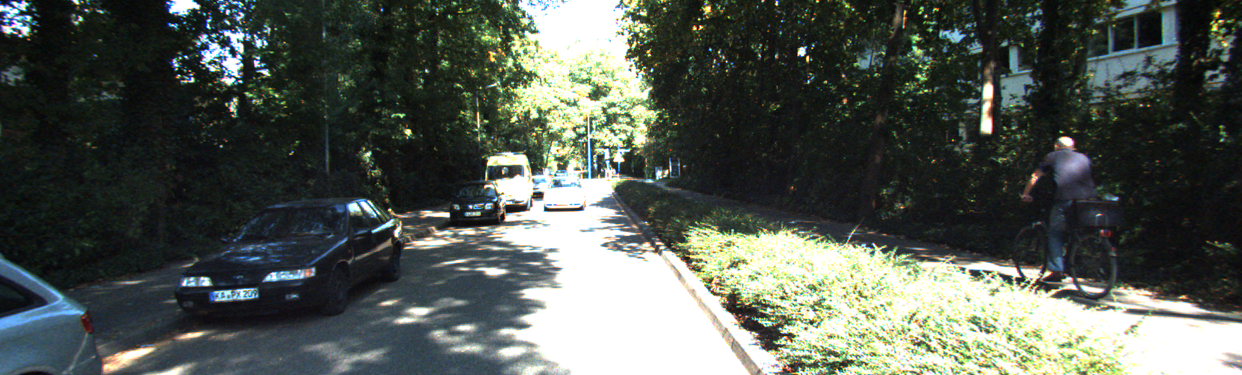
\includegraphics[width=0.66\linewidth]{imagenes/test_output_samples/input/2011_09_26_drive_0020_sync_0000000012.png}
}{2mm}{2mm}    
}
\hspace{-3mm}
    \subfloat{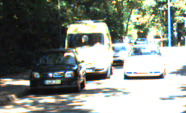
\includegraphics[width=0.33\linewidth]{imagenes/test_output_samples/input/2011_09_26_drive_0020_sync_0000000012_detail.png}}

\vspace{-3.5mm}

    \subfloat{\bottominset{\colorbox{white}{\textbf{(b)}}}{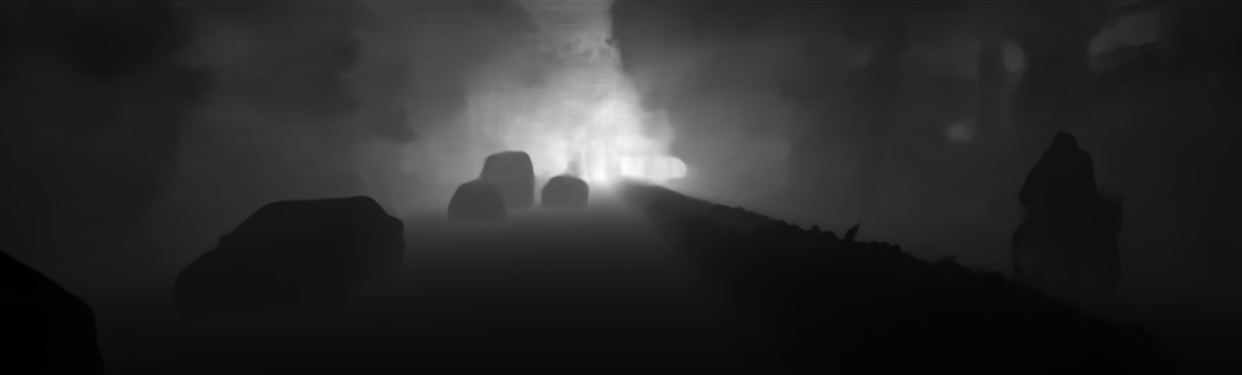
\includegraphics[width=0.66\linewidth]{imagenes/test_output_samples/2011_09_26_drive_0020_sync_0000000012/e7069aae.png}
}{2mm}{2mm}    
}
\hspace{-3mm}
    \subfloat{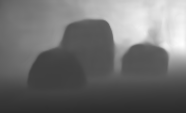
\includegraphics[width=0.33\linewidth]{imagenes/test_output_samples/2011_09_26_drive_0020_sync_0000000012/e7069aae_detail.png}}
    
\vspace{-3.5mm}

    \subfloat{\bottominset{\colorbox{white}{\textbf{(c)}}}{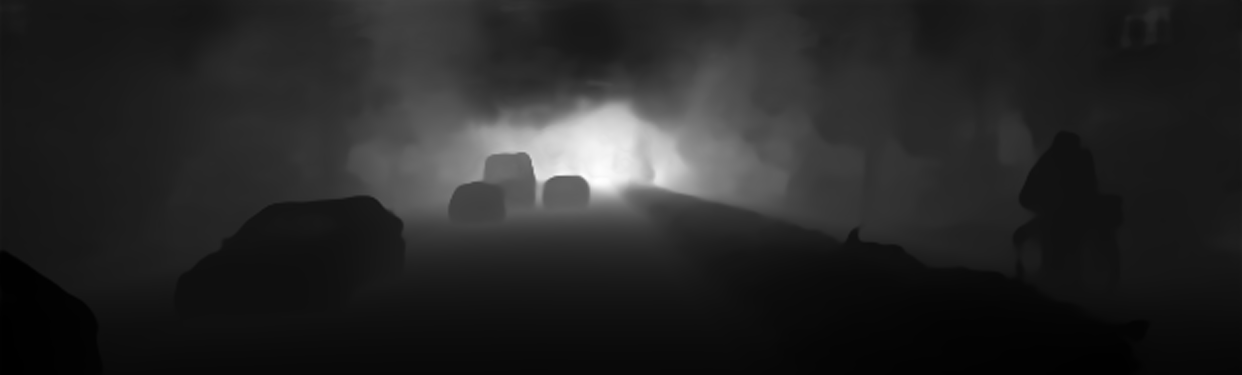
\includegraphics[width=0.66\linewidth]{imagenes/test_output_samples/2011_09_26_drive_0020_sync_0000000012/rdcufuen.png}
}{2mm}{2mm}    
}
\hspace{-3mm}
    \subfloat{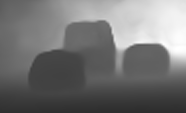
\includegraphics[width=0.33\linewidth]{imagenes/test_output_samples/2011_09_26_drive_0020_sync_0000000012/rdcufuen_detail.png}}
       
\caption{Resultados en función de la resolución de entrada. (a) Entrada del modelo y detalle. (b) Salida del modelo proporcionado en el repositorio de DPT \cite{visiontransformersDPT} (sin reducir la entrada). (c) Salida del modelo equivalente a DPT con el tamaño de entrada reducido.}
    \label{fig:cualitativa-1}
    % \end{figure}
% \captionsetup[subfigure]{labelformat=parens}





% \captionsetup[subfigure]{labelformat=empty}
   % \begin{figure}[!ht]
% \centering

    \subfloat{\bottominset{\colorbox{white}{\textbf{(a)}}}{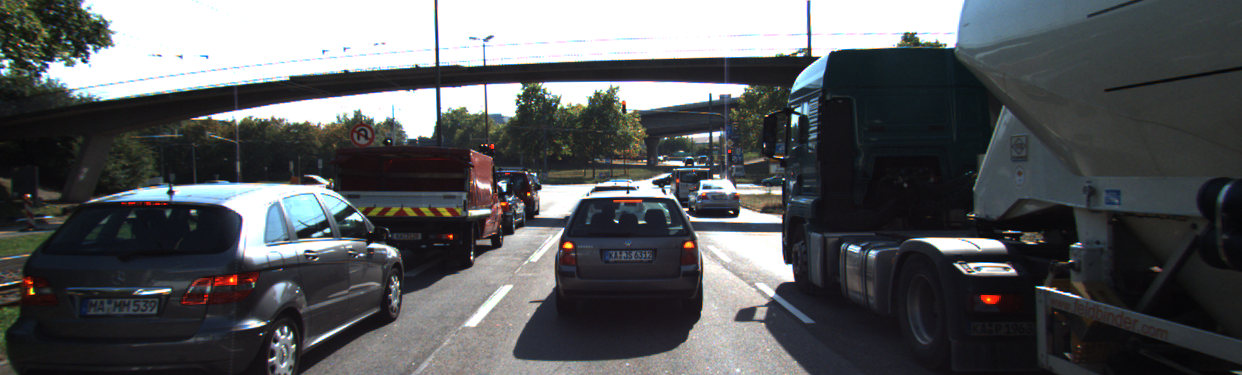
\includegraphics[width=0.66\linewidth]{imagenes/test_output_samples/input/2011_09_26_drive_0052_sync_0000000002.png}
}{2mm}{2mm}    
}
\hspace{-3mm}
    \subfloat{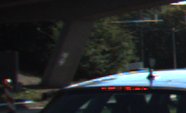
\includegraphics[width=0.33\linewidth]{imagenes/test_output_samples/input/2011_09_26_drive_0052_sync_0000000002_detail.png}}

\vspace{-3.5mm}

    \subfloat{\bottominset{\colorbox{white}{\textbf{(b)}}}{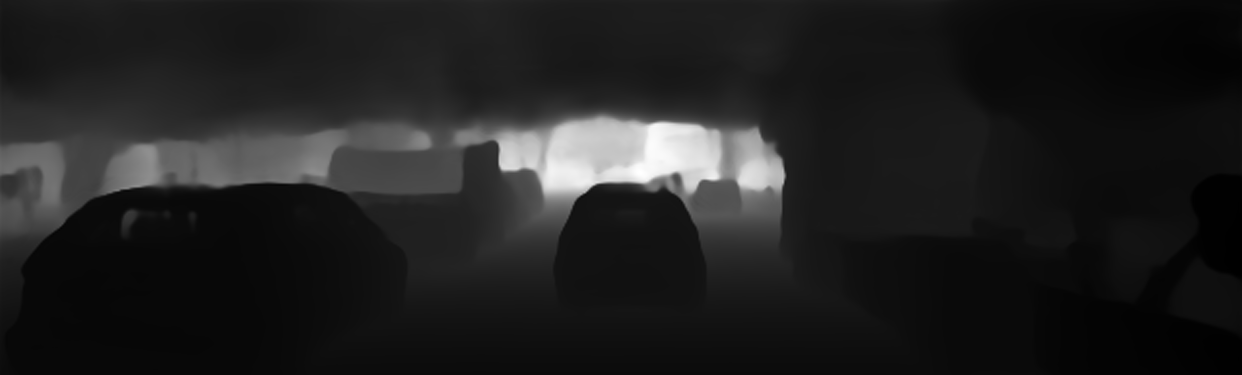
\includegraphics[width=0.66\linewidth]{imagenes/test_output_samples/2011_09_26_drive_0052_sync_0000000002/rdcufuen.png}
}{2mm}{2mm}    
}
\hspace{-3mm}
    \subfloat{
\includegraphics[width=0.33\linewidth]{imagenes/test_output_samples/2011_09_26_drive_0052_sync_0000000002/rdcufuen_detail.png}}
    
\vspace{-3.5mm}

    \subfloat{\bottominset{\colorbox{white}{\textbf{(c)}}}{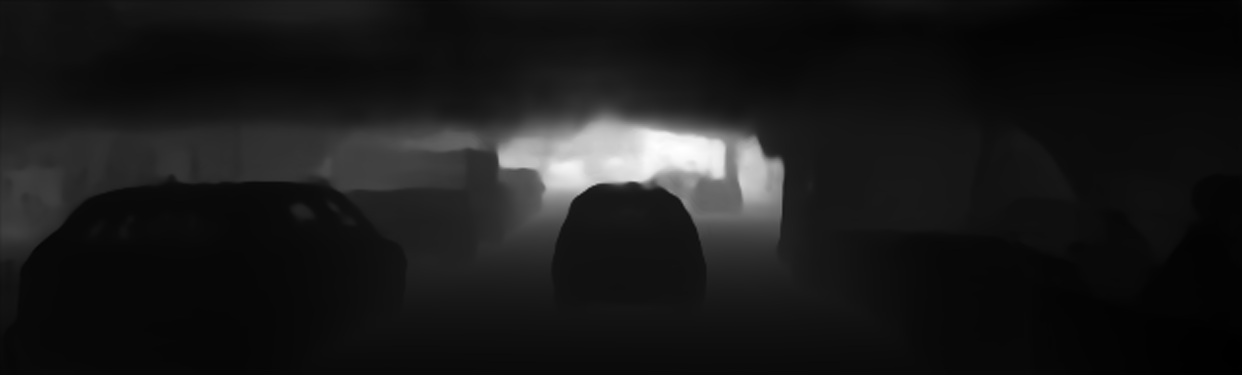
\includegraphics[width=0.66\linewidth]{imagenes/test_output_samples/2011_09_26_drive_0052_sync_0000000002/vulaigjq.png}
}{2mm}{2mm}    
}
\hspace{-3mm}
    \subfloat{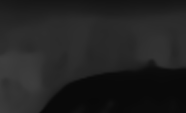
\includegraphics[width=0.33\linewidth]{imagenes/test_output_samples/2011_09_26_drive_0052_sync_0000000002/vulaigjq_detail.png}}
       
\caption{Resultados en función del \textit{backbone} empleado. (a) Entrada del modelo y detalle. (b) Salida del modelo equivalente a DPT con el tamaño de entrada reducido (ResNet50). (c) Salida del modelo equivalente a DPT con el tamaño de entrada reducido y EfficientNet-B0 como \textit{backbone}.}
    \label{fig:cualitativa-2}
    \end{figure}
\captionsetup[subfigure]{labelformat=parens}


En la \Cref{fig:cualitativa-3}, se encuentran las salidas de tres modelos que difieren en el número de cabezas de sus bloques de atención. En estas imágenes, sin embargo, es difícil apreciar diferencias, ya que como se ha visto en el \Cref{resultados-cuantitativos-cabezas}, la diferencia en las métricas en función de este parámetro es relativamente pequeña. A modo de detalle, se señala en el recorte de la derecha de esta Figura cómo la salida del modelo con una sola cabeza (c), estima incorrectamente la profundidad en el reflejo del lateral de la camioneta, mientras que los otros dos modelos sí que lo identifican correctamente.






\captionsetup[subfigure]{labelformat=empty}
    \begin{figure}[!ht]
\centering

    \subfloat{\bottominset{\colorbox{white}{\textbf{(a)}}}{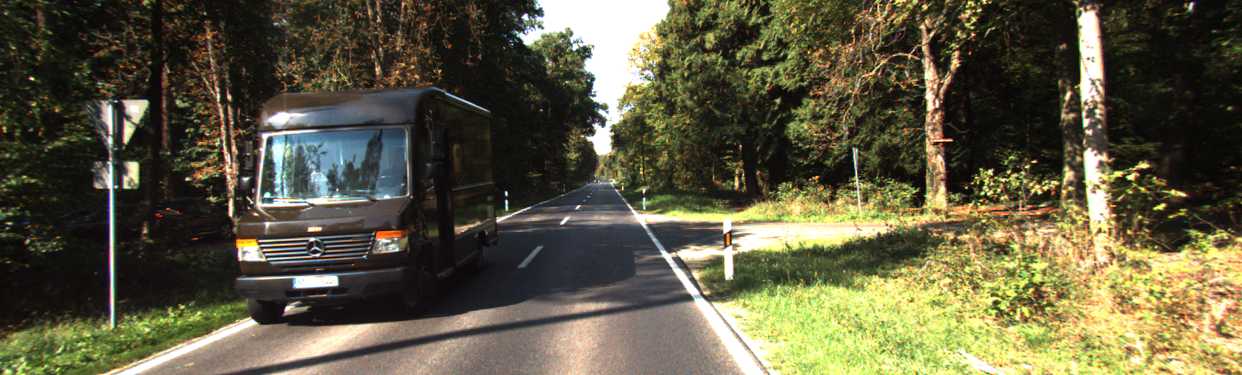
\includegraphics[width=0.66\linewidth]{imagenes/test_output_samples/input/2011_09_26_drive_0027_sync_0000000056.png}
}{2mm}{2mm}    
}
\hspace{-3mm}
    \subfloat{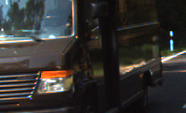
\includegraphics[width=0.33\linewidth]{imagenes/test_output_samples/input/2011_09_26_drive_0027_sync_0000000056_detail.png}}

\vspace{-3.5mm}

    \subfloat{\bottominset{\colorbox{white}{\textbf{(b)}}}{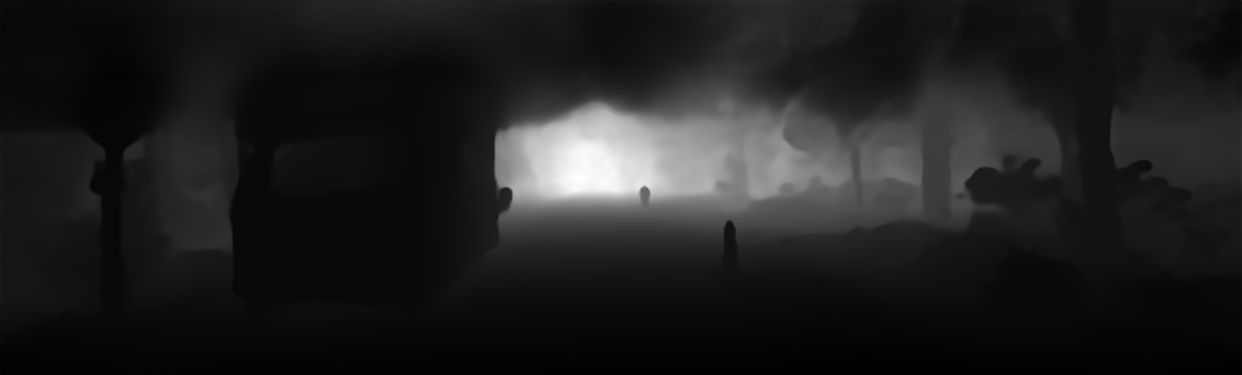
\includegraphics[width=0.66\linewidth]{imagenes/test_output_samples/2011_09_26_drive_0027_sync_0000000056/rdcufuen.png}
}{2mm}{2mm}    
}
\hspace{-3mm}
    \subfloat{
\includegraphics[width=0.33\linewidth]{imagenes/test_output_samples/2011_09_26_drive_0027_sync_0000000056/rdcufuen_detail.png}}
    
\vspace{-3.5mm}

    \subfloat{\bottominset{\colorbox{white}{\textbf{(c)}}}{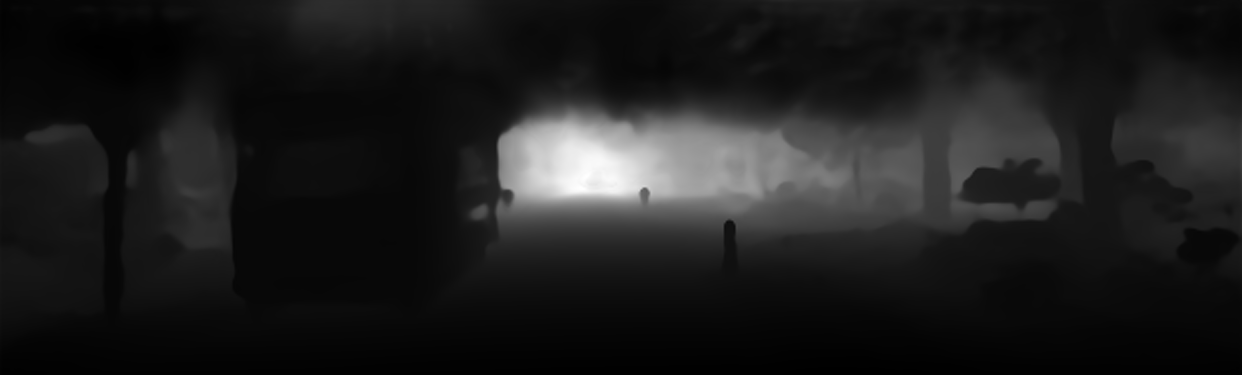
\includegraphics[width=0.66\linewidth]{imagenes/test_output_samples/2011_09_26_drive_0027_sync_0000000056/ohegkkpv.png}
}{2mm}{2mm}    
}
\hspace{-3mm}
    \subfloat{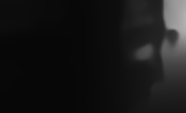
\includegraphics[width=0.33\linewidth]{imagenes/test_output_samples/2011_09_26_drive_0027_sync_0000000056/ohegkkpv_detail.png}}
    
\vspace{-3.5mm}

    \subfloat{\bottominset{\colorbox{white}{\textbf{(d)}}}{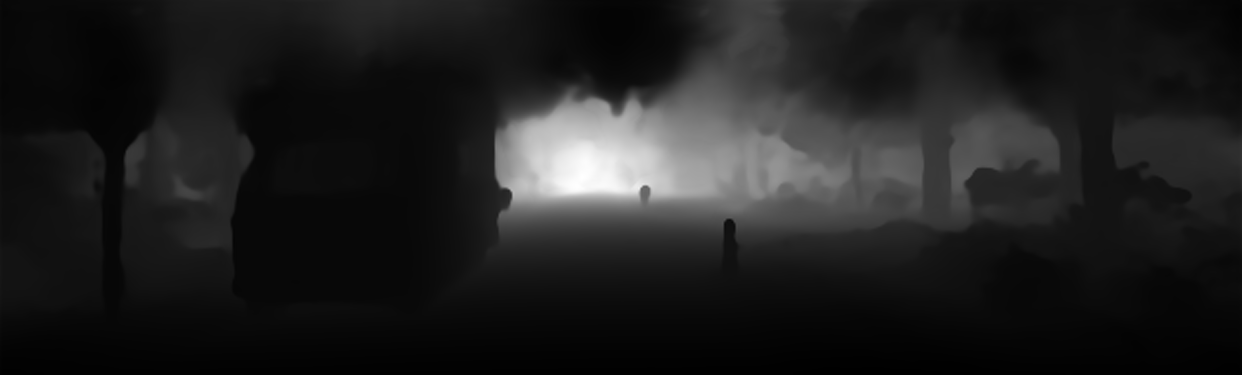
\includegraphics[width=0.66\linewidth]{imagenes/test_output_samples/2011_09_26_drive_0027_sync_0000000056/ytsftbhm.png}
}{2mm}{2mm}    
}
\hspace{-3mm}
    \subfloat{\includegraphics[width=0.33\linewidth]{imagenes/test_output_samples/2011_09_26_drive_0027_sync_0000000056/ytsftbhm_detail.png}}
       
\caption{Resultados en función del número de cabezas de atención del modelo. (a) Entrada del modelo y detalle. (b) Salida del modelo equivalente a DPT con el tamaño de entrada reducido (12 cabezas de atención). (c) Salida del modelo equivalente a DPT con el tamaño de entrada reducido y 1 cabeza de atención. (d) Salida del modelo equivalente a DPT con el tamaño de entrada reducido y 24 cabezas de atención.}
    \label{fig:cualitativa-3}
    \end{figure}
\captionsetup[subfigure]{labelformat=parens}

\pagebreak




En el caso de la \Cref{fig:cualitativa-5}, es posible comparar las salidas de dos modelos cuya única diferencia es el mecanismo de atención empleado. En este caso, de forma similar al cambio del número de cabezas, es difícil observar diferencias notables. A modo de detalle, y en contra de lo que indican las métricas en el conjunto de validación, es posible observar como el modelo con la atención estándar (b) predice una profundidad errónea para el coche del reflejo del cristal de un edificio, mientras que el modelo con el mecanismo de atención del \textit{Performer} si que identifica correctamente la pared.










\captionsetup[subfigure]{labelformat=empty}
    \begin{figure}[!ht]
\centering

    \subfloat{\bottominset{\colorbox{white}{\textbf{(a)}}}{\includegraphics[width=0.66\linewidth]{imagenes/test_output_samples/input/2011_09_26_drive_0048_sync_0000000018.png}
}{2mm}{2mm}    
}
\hspace{-3mm}
    \subfloat{\includegraphics[width=0.33\linewidth]{imagenes/test_output_samples/input/2011_09_26_drive_0048_sync_0000000018_detail.png}}

\vspace{-3.5mm}

    \subfloat{\bottominset{\colorbox{white}{\textbf{(b)}}}{\includegraphics[width=0.66\linewidth]{imagenes/test_output_samples/2011_09_26_drive_0048_sync_0000000018/rdcufuen.png}
}{2mm}{2mm}    
}
\hspace{-3mm}
    \subfloat{\includegraphics[width=0.33\linewidth]{imagenes/test_output_samples/2011_09_26_drive_0048_sync_0000000018/rdcufuen_detail.png}}
    
\vspace{-3.5mm}

    \subfloat{\bottominset{\colorbox{white}{\textbf{(c)}}}{\includegraphics[width=0.66\linewidth]{imagenes/test_output_samples/2011_09_26_drive_0048_sync_0000000018/mdfjfbjy.png}
}{2mm}{2mm}    
}
\hspace{-3mm}
    \subfloat{\includegraphics[width=0.33\linewidth]{imagenes/test_output_samples/2011_09_26_drive_0048_sync_0000000018/mdfjfbjy_detail.png}}
       
\caption{Resultados en función de los \textit{hooks} empleados. (a) Entrada del modelo y detalle. (b) Salida del modelo equivalente a DPT con el tamaño de entrada reducido (atención estándar). (c) Salida del modelo equivalente a DPT con el tamaño de entrada reducido y atención tipo \textit{Performer}.}
    \label{fig:cualitativa-5}
    \end{figure}
\captionsetup[subfigure]{labelformat=parens}

\pagebreak


Por último, en la \Cref{fig:cualitativa-4}, lo que cambia en los modelos son los \textit{hooks} en los bloques de atención, y por lo tanto está directamente relacionada con el \Cref{resultados-cuantitativos-hooks}. En estas salidas, sí que es posible visualizar como los resultados son peores en algunos detalles, sobre todo en objetos de menor tamaño en la imagen como son las señales de tráfico señaladas en el detalle de la derecha o los carteles más alejados.






\captionsetup[subfigure]{labelformat=empty}
    \begin{figure}[!ht]
\centering

    \subfloat{\bottominset{\colorbox{white}{\textbf{(a)}}}{\includegraphics[width=0.66\linewidth]{imagenes/test_output_samples/input/2011_09_26_drive_0029_sync_0000000196.png}
}{2mm}{2mm}    
}
\hspace{-3mm}
    \subfloat{\includegraphics[width=0.33\linewidth]{imagenes/test_output_samples/input/2011_09_26_drive_0029_sync_0000000196_detail.png}}

\vspace{-3.5mm}

    \subfloat{\bottominset{\colorbox{white}{\textbf{(b)}}}{\includegraphics[width=0.66\linewidth]{imagenes/test_output_samples/2011_09_26_drive_0029_sync_0000000196/rdcufuen.png}
}{2mm}{2mm}    
}
\hspace{-3mm}
    \subfloat{\includegraphics[width=0.33\linewidth]{imagenes/test_output_samples/2011_09_26_drive_0029_sync_0000000196/rdcufuen_detail.png}}
    
\vspace{-3.5mm}

    \subfloat{\bottominset{\colorbox{white}{\textbf{(c)}}}{\includegraphics[width=0.66\linewidth]{imagenes/test_output_samples/2011_09_26_drive_0029_sync_0000000196/bqaauynr.png}
}{2mm}{2mm}    
}
\hspace{-3mm}
    \subfloat{\includegraphics[width=0.33\linewidth]{imagenes/test_output_samples/2011_09_26_drive_0029_sync_0000000196/bqaauynr_detail.png}}
    
\vspace{-3.5mm}

    \subfloat{\bottominset{\colorbox{white}{\textbf{(d)}}}{\includegraphics[width=0.66\linewidth]{imagenes/test_output_samples/2011_09_26_drive_0029_sync_0000000196/paqfhvde.png}
}{2mm}{2mm}    
}
\hspace{-3mm}
    \subfloat{\includegraphics[width=0.33\linewidth]{imagenes/test_output_samples/2011_09_26_drive_0029_sync_0000000196/paqfhvde_detail.png}}
       
\caption{Resultados en función de los \textit{hooks} empleados. (a) Entrada del modelo y detalle. (b) Salida del modelo equivalente a DPT con el tamaño de entrada reducido (\textit{hooks} en bloques $[8, 11]$). (c) Salida del modelo equivalente a DPT con el tamaño de entrada reducido y \textit{hooks} en los bloques $[2, 5]$. (d) Salida del modelo equivalente a DPT con el tamaño de entrada reducido y \textit{hooks} en los bloques $[0, 1]$.}
    \label{fig:cualitativa-4}
    \end{figure}
\captionsetup[subfigure]{labelformat=parens}








\clearpage